\documentclass[11pt,a4paper]{memoir}
\usepackage[utf8]{inputenc}
\usepackage[pdftex]{graphicx}	
\usepackage{amsmath}
\usepackage[table,xcdraw]{xcolor}
\usepackage[export]{adjustbox}
\usepackage{changepage}
\usepackage{caption}
\usepackage{subcaption}
\usepackage[english]{babel}
\numberwithin{figure}{section}
\numberwithin{table}{section}
\numberwithin{equation}{section}

\usepackage{lscape}
\usepackage[a4paper, 
left=1.25in, right=1.25in, top=1.25in, bottom = 1in, footskip=.5in, headsep=.5in]{geometry}
\usepackage{makeidx}
\makeindex


\begin{document}
\frontmatter

\thispagestyle{empty}
\begin{center}


	
\includegraphics[width=0.8\textwidth]{upotrofies_uni.jpg}\par\vspace{1cm}
	{\scshape\Large A Thesis Submitted for Master of Science in \par}
        
    {\scshape\Large Bioinformatics\par}
    \vspace{0.5cm}
    {\scshape\Large In Collaboration with BioMediq\par}

	\vspace{1cm}
	{\huge\bfseries A Comparison of 2D and 3D Convolutional Neural Networks for Knee Cartilage  Segmentation in MRI  \par}
	\vspace{1.5cm}
	{\Large\itshape Joseph Blair\par}
 
	\vfill
	Supervised by\par
	~ Prof. Christian \textsc{Igel}\par
    \vfill
    Industrial Supervisor\par
    ~ Erik \textsc{Dam}
    

	\vfill

% Bottom of the page
	{\large \today\par}
    \end{center}

\chapter*{Abstract}
Knee osteoarthritis is a complex disease affecting the bone and cartilage of the knee joint, particularly in the elderly and obese, making it increasingly important to quickly and accurately diagnose the disease. \\ 

Advances in medical imaging have made it much easier to study diseases and to identify key biomarkers aiding diagnosis and possible prognoses. With increasing amounts of image data available for research, and increased computing power, it has also been possible to use machine learning for the identification of new biomarkers and to aid diagnosis. Part of this process, particularly when looking at osteoarthritis, is the segmentation of specific regions of interest or pathology, such as cartilage, in medical images. \\

This thesis investigates three different approaches of cartilage segmentation from MRI scans using convolutional neural networks (CNNs). These are deep neural networks with several layers of processing, some of which convolve their input with linear filters. The three-dimensional nature of MRI scans naturally lead to full 3D convolutional networks, segmenting images in a patch wise fashion, however at a high computation cost. Planar, and tri-planar approaches were also explored, in which 2D convolutions were performed on patches extracted from axial, coronal and saggital slices centred around the voxel to be classified. Here performance was evaluated as well as the temporal demands of each of the methods.\\

The tri-planar network was found to have the best segmentation accuracy, achieving a mean Dice-Sørensen score of 0.8707 $\pm0.0474$. This methodology significantly improved on State-of-the-art methods (P-Value \textless 0.0001) evaluated on the same dataset. An entry into the IWOAI 2016 Segmentation Challenge was also presented, in which a 3D CNN deep learning framework placed third amongst multi-atlas based approaches.


\chapter*{Acknowledgements}
I would like to express my gratitude to my industrial supervisor Erik Dam for his continuous support, insights and guidance for the duration this project. I would also like to thank him for providing me with his own image processing and visualisation tools which made this project possible. Furthermore I would like to thank Christian Igel my academic supervisor for his valuable inputs he has provided during the course of this project. Finally, I would like to thank all the employees of BioMediq for welcoming me into their organisation, and for making the process of this master's thesis thoroughly enjoyable.

\clearpage

\begin{KeepFromToc}
 \textsc{ \tableofcontents}
\end{KeepFromToc}
\clearpage
\begin{KeepFromToc}
\listoffigures
 \end{KeepFromToc}
 \clearpage
 \begin{KeepFromToc}
\listoftables
 \end{KeepFromToc}

\mainmatter
\chapter{Introduction}

Due to the rapid increase in availability of medical data and image data through recent digitalisation processes, it has been made possible to design, and apply algorithms for analysis to give some clinical insight. Deep learning techniques, having proven success in other fields, are now being used on medical data to aid doctors in decision making.\\

This report will give an overview of deep learning concepts, their application, and a more in depth look at convolutional neural networks. An overview of osteoarthritis (OA) of the knee shall also be given, a multifaceted musculo-skeletal disease. In order to investigate this disease, MRI scans which allow the visualisation of soft tissue, can be computationally analysed. In the case of osteoarthritis, the main regions affected by OA are the femoral and tibial cartilage, which decrease in volume with progression of the disease\cite{Conaghan2011SummaryGroup.}. \\

This thesis is concerned with the application of deep learning methodologies to the problem of medical image segmentation. This is a problem which has been approached before by many groups such as in \cite{Avendi2016AMRI}, \cite{Zhang2015DeepSegmentation} and \cite{Liao2013RepresentationSegmentation}.\\

Finally the results of experimental work carried out over the course of this thesis will be presented. The objectives of these experiments were to compare three different convolutional network architectures for the segmentation of cartilage of the knee, whilst improving on existing image segmentation methodologies. These methods use a variety of different methodologies such as multi-atlas methodologies \cite{Shan2012AUTOMATICIMAGES.}, or existing deep learning approaches \cite{Prasoon2013DeepNetwork}.\\

The results of the IWOAI 2016 Segmentation Challenge \cite{2016InternationalChallenge} will also be presented, to which a submission was made at an early stage of the research process.


\chapter{Deep Learning and Convolutional Networks}
Since the 1940's the field of research of Neural Networks has been aiming to mimic the way in which the human brain processes information, in order to perform human-like tasks such as speech and pattern recognition, modelling and prediction  \cite{VanDerSmagt1996AnNetworks}. Although there were some early successes in the field of artificial intelligence which achieved this \cite{Carpenter1989NeuralMemory}\cite{Lippmann1989ReviewRecognition}, it wasn't until the early 2000's that neural networks, and in particular deep learning, driven mainly by Geoffrey Hinton really began to excel \cite{Hinton2006ANets.}. Artificial Neural Networks have now been used widely both commercially for example in security systems \cite{Korkmaz2016DevelopingSystems} and financial forecasting software \cite{Barunik2016ForecastingNetworks}, and are starting to become more prevalent in more scientific and medical contexts \cite{Zribi2016NeuralMaking}. \\

Although an overview of "traditional" neural networks (NN's) is slightly out of the scope of this report, a more in depth description of them can be found in \cite{Goodfellow-et-al-2016-Book}. Traditional neural networks tend be be comprised of one or two layers of neurons, and work in a "supervised" manner to solve classification and regression tasks \cite{Goodfellow-et-al-2016-Book}. The neurons in each layer use a non-linear function to transform a multidimensional-input into a single output. Deep Learning is a more recent concept which utilises many more layers, and is in essence a combination of machine learning algorithms used to tackle both supervised and unsupervised problems \cite{LeCun2015DeepLearning}.\\

In this section, we will look at the use of Deep Learning techniques, and in particular convolutional neural networks (CNNs).  

\section{An Overview of Deep Learning}
As briefly mentioned above, Deep Learning frameworks are formed of many layers of neurons which are designed to learn distinguishable features to help solve a given problem \cite{LeCun2015DeepLearning}.  Each layer learns features from previous layers in the network, resulting in high levels of abstraction \cite{Egmont-Petersen2002ImageReview} which can be required with certain complicated functions such as computer vision and speech recognition tasks. \\

The application of Deep Learning architectures has had a great deal of success in the application of image recognition and analysis \cite{Goodfellow2013Multi-digitNetworks} and the understanding of text \cite{Mikolov2013ExploitingTranslation}. Deep Learning is comprised of different types of networks such as Recurrent Neural Networks (RNNs) and Convolutional Neural Networks (CNNs). The former, are mainly used for sequence analysis concerning speech, text as well as biological sequences \cite{Graves2013SpeechNetworks} \cite{Alipanahi2015}. The latter, which we shall be focussing on here, have been mainly used for image and video analysis, although also has had application in sequence analysis.

\section{Convolutional Neural Networks}

As with other, more traditional Neural Network concepts, Convolutional Neural Networks take inspiration from biological principles in their design, and more specifically, claim to mimic the visual cortex. In particular, this is in line with the locally selective neurons seen in mammalian vision systems, discovered by Hubel and Wiesel's in the 1960's \cite{HUBEL1962}. \\

Convolutional networks, although were explored previously by, among others, Graupe et al.\cite{Graupe1988ApplicationsProcessing}, were properly established by LeCun et al.\cite{LeCun2015DeepLearning}, and have now been broadly applied to 2D and 3D image and video data, and more recently also used for natural language processing and sequence data analysis. Some existing work has been done on the segmentation of medical images using deep learning which is what we shall explore in this report. For example, Kleesiek et al. used deep neural networks for the skull stripping in brain MRI scans \cite{Kleesiek2016DeepStripping}. Havaei et al. also used deep networks for the segmentation of tumours in brain MRI scans \cite{Havaei2017BrainNetworks}. \\

They employ three key mechanisms which make them differ form traditional neural networks; local receptive fields, weight sharing and sub-sampling. These mechanisms aid the building of a model which is invariant to translation, and can provide information regarding the spatial structure of the input.

\subsection{Convolutional Layers}

Convolutional layers act by detecting features located in subsets of the input data, which is most often an image \cite{Lecun1998Gradient-basedRecognition}. In this subset (usually square in shape), a local receptive field, all pixels or voxels will be connected to one neuron. Each connection from the voxel to the neuron will learn a weight dependant on its receptive field. The neuron these are connected to will learn a bias over all these weights. This can be seen in Figure \ref{fig:CNN}. For an input image, the local receptive field is moved across the input, until all pixels or voxels haven been seen. \\

\begin{figure}[!h]
\centering
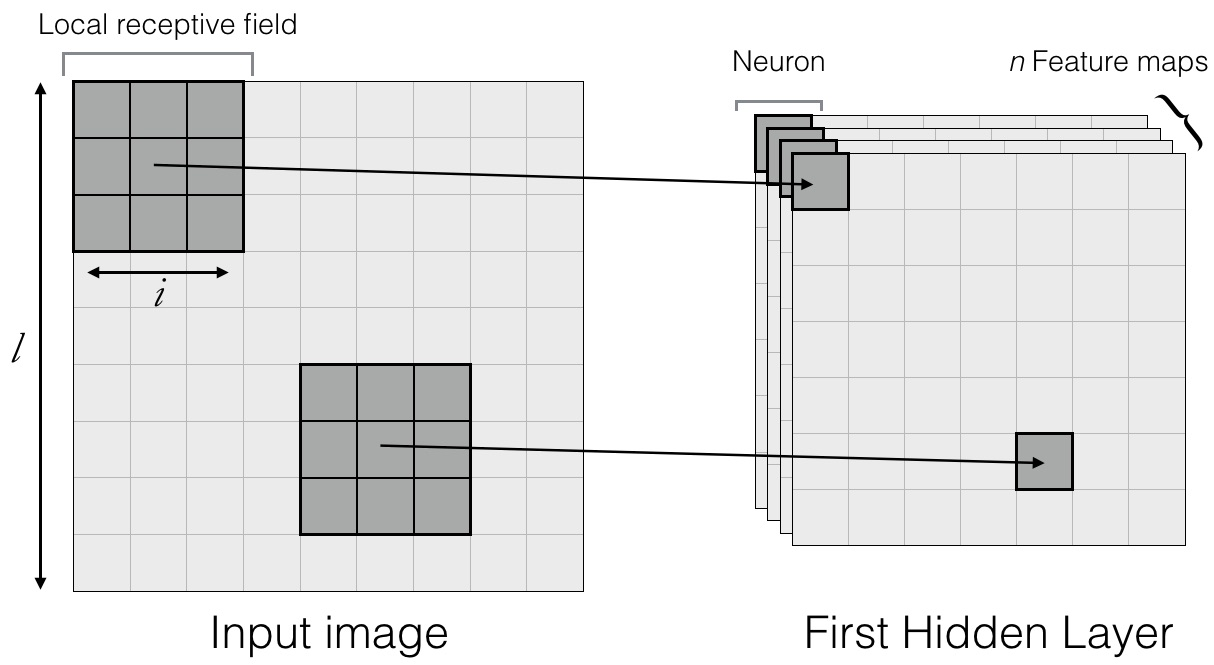
\includegraphics[width=1\textwidth]{CNN.jpg}
\caption[Illustration of feature map generation in a convolutional layer]{Illustration depicting the formation of feature maps through a convolutional layer. A filter, or local receptive field of a given size, in this case 3x3, passes over the input generating one node for every position it occupies. This results in a feature map of width ($l - (i-1)$), where $l$ is the width of the square input and $i$ the width of the filter.}
\label{fig:CNN}
\end{figure}

It is also important to mention that the weights for all hidden neurons are shared, meaning all neurons in a group learn the same feature \cite{RanzatoMarcAurelio2007UnsupervisedRecognition}. This group of neurons is known as a feature map for that layer. Many feature maps can be generated for each layer, with each map learning a different set of feature weights. As each feature map contains information pertaining to all local receptive fields, and hence every pixel in the input, the features being learnt are not dependent on the location in the image. This gives some translation invariance in the network, and allows a feature to be found at any position in the image. By using this shared weight strategy, the efficiency of weight learning is also much greater, due to a reduction in the number of free parameters needed to be learnt. This lowers the degrees of freedom of the generated model, allowing better generalisation across the feature maps. This can be seen in Figure \ref{fig:WShare}. \\

\begin{figure}[!h]
\centering
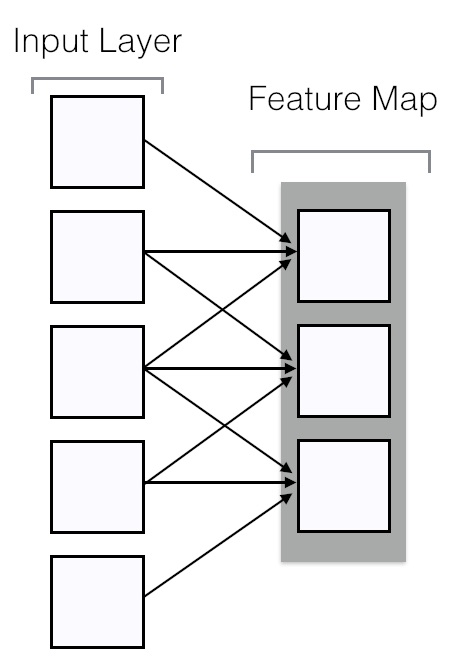
\includegraphics[scale=0.25]{WS.jpg}
\caption[Illustration of weight sharing in a convolutional neural network]{Illustration depicting the sharing of weights within a feature map for a set of input neurons of 1 dimension. Each neuron in the feature map receives inputs from the receptive field, in this case $3*1$ in size, with a stride size of 1. All neurons in the feature map share the same weights, and so are trained for the same feature.}
\label{fig:WShare}
\end{figure}

This can be used over 1D, 2D or 3D matrices, depending on the shape of the input vector. Each feature map will also have the same dimensionality on the input.\\

The activation function used by each layer can vary, and much research has been put into optimising this. As shown by Maas et al.\cite{Maas}, Rectified Linear Activation Function (ReLu) can be far superior to more traditional activation functions such as Sigmoidal and tanh, in that it can accelerate convergence of gradient descent. The ReLu function \cite{Maas} is given by $y = max(0, x)$.  This is now very commonly used in deep-learning frameworks, and will be employed in experiments described in this report.

\subsection{Pooling and Maxpooling Layers}
As previously mentioned, sub-sampling, also plays a large part in the performance of CNNs and aids with spatial invariance \cite{RanzatoMarcAurelio2007UnsupervisedRecognition}. Sub-sampling is employed in the form of pooling layers, which are usually used immediately after a convolutional layer. A pooling layer condenses the output from a convolutional layer, by generalising regions within the feature map. Maxpooling or pooling layers divide the output from the previous layer into no-overlapping regions (usually square). The maximum value of a region of the feature map, is then used in the condensed feature map. A simple pooling layer uses the same process, however outputs the mean of each region rather than the maximum. An illustration of this can be seen in Figure \ref{fig:MPool}. Having reduced the resolution of the feature maps, these pooling layers help provide a form of translation invariance, as well as lowering computational demand. 

\begin{figure}[!h]
\centering
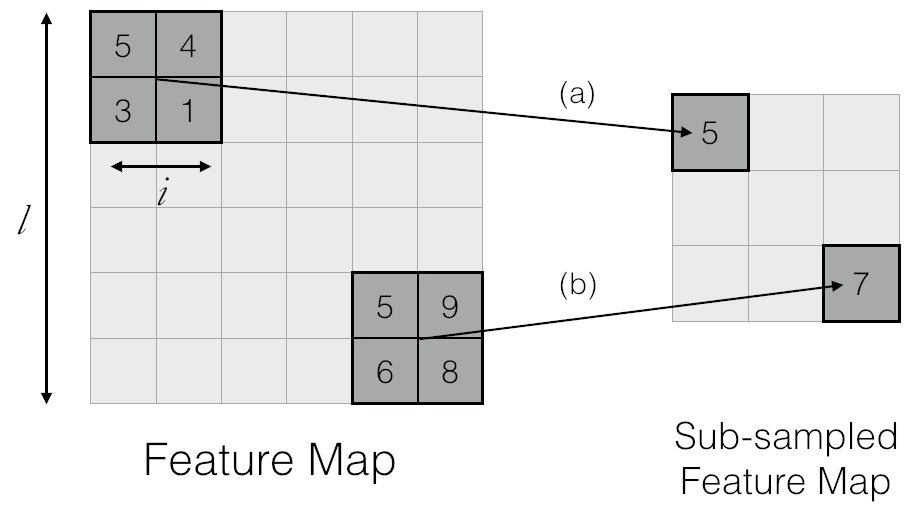
\includegraphics[scale=0.37]{MPool.jpg}
\caption[Illustration of a pooling and maxpooling operation in a convolutional neural network ]{Illustration showing (a) a maxpooling operation in which a $2*2$  window convolves a feature map, with the maximum value in the appearing sub-sampled output, and (b) a pooling operation in which all voxels in a $2*2$ window are averaged, with the mean value appearing in the corresponding location in the sub-sampled map. Here the resulting size of the sub-sampled feature map is ($ l /i$) where $l$ is the width of the square input and $i$ is the width of the pooling window. Partial pooling windows are often discarded.}
\label{fig:MPool}
\end{figure}


\subsection{Dense Layers and Concatenation}
Following a series of convolutional and pooling layers, a fully connected layer completes high level analysis of the input \cite{Goodfellow-et-al-2016-Book}. Fully connected layers take every input from the previous layer, and connect them to every neuron it has available. The output from this is then fed into an output layer. In classification problems, this output layer will very often use a softmax function to "squash" the weights into a $k$-dimensional vector, where $k$ is equal to the number of classes being classified. \\

These layers can be merged in the case that there should be the need to bring many networks together. This can be done by either concatenation in which they will be "stacked" across one dimension, or summed along one axis. In order for both of these to be possible the dimensions of the weights from the dense layer must match. 

\subsection{Dropout Layers}
Dropout layers may sometimes be used as a form of regularisation in neural networks in order to help prevent overfitting \cite{Hinton2012ImprovingDetectors}. This works by preventing neurons from 'co-adapting', which occurs when a feature detector is only useful in combination with certain other feature detectors present.\\

A drop out is performed by disabling a percentage of the neurons in a dense layer, forcing the remaining active neurons to generalise the inputs.

\subsection{Loss and Training Functions} 
Following a forward pass of a convolutional network (from input to output), the outputs must be evaluated with a loss function, before the weights are updated. When updating the weights of a network, either a gradient-based or non-gradient based method can be used. Here we shall only look at gradient based methods.  

With $x$  as our input, and $y$ our target, or label for $x$, gradient based methods look to find the weights, which are able to minimise the difference between $x$ and $y$. In order to do this, one must first use a loss function to quantify the difference between the input and target. A commonly used loss function is \cite{DeBoer2005AMethod} categorical cross entropy \\

\begin{eqnarray} 
  C(y, a) = -\frac{1}{n} \sum_x \left[y \ln a + (1-y ) \ln (1-a) \right] 
  \label{eq:cross}\enspace,
\end{eqnarray}

where $a$ is the activation output, and $n$ is number of samples in the training batch. \\

Following the evaluation of the training batch using a loss function, it is then possible to start optimisation using gradient descent. There are many different variations of gradient descent optimisation algorithms, which all have the same goal. An example of this is \cite{nesterov1983method} Nesterov's Accelerated Gradient descent 

\begin{eqnarray}
V_{t+1} = \mu V_t - \alpha \nabla L(W_t + \mu V_t) \enspace,
\label{eq_nest}
\end{eqnarray}

\begin{eqnarray}
W_{t+1} = W_t + V_{t+1} \enspace,
\label{update}
\end{eqnarray}

where the aim is to obtain the update value, $V_{t+1}$ and the updated weights $W_{t+1}$. This is computed with the hyper-parameters $\mu$, the momentum and $\alpha$ the learning rate. This differs from standard Stochastic gradient descent in that the gradient is taken on the weights with added $\mu$, rather than just the weights. \\

The importance of using momentum when training a network was shown by \cite{SutskeverOnLearning}, and shall be used in this report. The issue which can arise with gradient based methods such as this, is that learning rates and momentum magnitude must be chosen prior to training. If they are not selected properly, it can cause one to be stuck in a local-minima or to take a very long time to converge. \\

\subsection{Why use CNN's}
As mentioned in previous sections, convolutional networks have various properties which make them differ from traditional feed forward neural networks; weight sharing, sub-sampling and local receptive fields. These make them particularly powerful when using large input data, or data with high dimensionality such as image or video data. Traditional neural networks connect every input neuron to a hidden neuron, creating extremely high number of parameters.\\

If we consider a relatively small input image of $25^2$, equating to 625 input neurons ($25*25$), with a fully connected hidden layer with 40 hidden neurons, a total of 25,000 parameters will need to be optimised ($625 * 40$), plus 40 biases. In contrast to this, the same image in a convolutional network, with a local receptive field (or filter) size of $5^2$, one feature map will have a total of 25 shared weights($5 *5$). If we consider having 40 feature maps here, this layer will have a total of 1,000  parameters to optimise ($25 * 40$). \\

With such a high number of parameters, as seen in fully connected networks, optimisation becomes very difficult, and can be very prone to over-fitting. By using weight sharing, the number of parameters are greatly reduced, avoiding this problem, and also reducing computational complexity.\\

\clearpage

\chapter{Osteoarthritis}
\section{Osteoarthritis and Knee Anatomy}
Osteoarthritis (OA) is a degenerative and often progressive musculo-skeletal disease, and is the most widely spread musculo-skeletal disease worldwide \cite{Lawrence2008}. The elderly population is the most affected, with over 50\% of over 65's globally, showing signs of osteoarthritis. Age is the strongest risk factor of OA, however is also commonly seen in the obese, and those with high levels of trauma \cite{Glyn-Jones2015}. \\

Osteoarthritis causes pain and swelling in the joints of sufferers and often leads to loss of mobility. With a growing elderly and obese population in the western world, the financial demand placed on health and welfare systems to combat the disease is increasing. All this calls for improvements in diagnosis and treatment to help reduce this impact \cite{Zhang2010EpidemiologyOsteoarthritis.}.  \\

Osteoarthritis can occur in any joint of the body, but is most commonly seen in the knees, hips, lower back and fingers of patients. The development of the disease is multifaceted, with bio-mechanical, biological and genetic traits, all contributing to its occurrence. As with any form of OA, osteoarthritis of the knee is complex. As can be seen from Figure \ref{fig:Knee}, the knee is comprised of two large bones, the femur, a larger bone forming the upper part of the leg, and the tibia forming the lower part of the leg. Cartilage, a smooth fibrous tissue,  articulates both femur and tibia bones where they join, which is split into lateral and medial sides \cite{Majumdar2010AdvancesOsteoarthritis}.  \\

\begin{figure}[h]
\centering
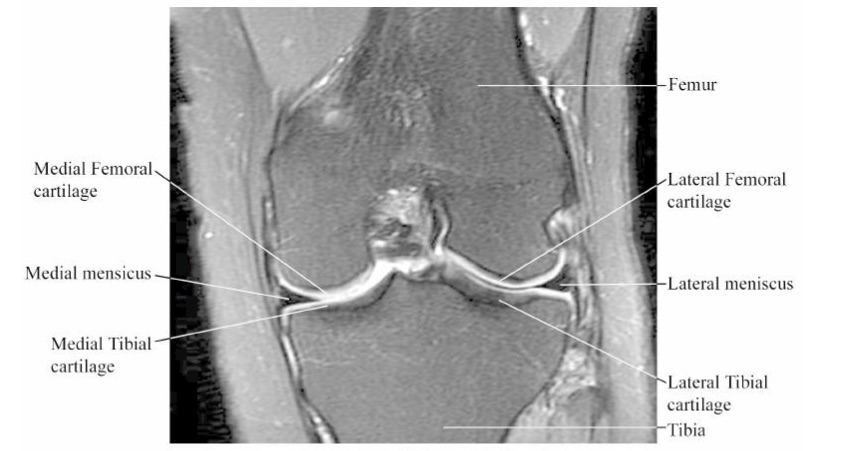
\includegraphics[scale=0.4]{knee_anatomy.jpg}
\caption[Knee anatomy shown in a saggital slice of a knee MRI scan ]{Coronal T2-weighted Magnetic Resonance Image displaying the knee and selected surrounding structures, adopted from Majumdar, 2010 \cite{Majumdar2010AdvancesOsteoarthritis}}
\label{fig:Knee}
\end{figure}

The main pathological effects of osteoarthritis are those of both tibial and femoral cartilage, which will show signs of wear and degradation \cite{Cicuttini2001}. Typically there will also be a change in trabecular structure (osseous tissue found near the end of the bone), and osteophyte formation visible in a patient diagnosed with osteoarthritis \cite{Eckstein2009}. Each of these physiological attributes are not unique to OA, but all play a part in the development of the disease. The disease is graded by severity according to the Kellgren-Lawrence scale, and ranges from 0, a healthy knee to 4, an extreme case in which severe sclerosis, osteophyte formation and clear bone deformity can be seen \cite{Schiphof2008DifferencesOsteoarthritis.}.

\section{Current Diagnosis and Research}
New methods of diagnosis and treatment are constantly being researched in order to improve accuracy and speed of the procedures. At present there is no real treatment for the disease beyond more than pain relief \cite{Dieppe2011}. A more thorough understanding of the development and clinical aspects of the disease will likely aid the development of successful treatments to help prevent or treat the disease.  \\ 

Currently, doctors use various methods to identify presence of osteoarthritis in patients. The primary diagnostic markers used in the diagnosis of OA are pain, discomfort and often a loss of function observed in the patient \cite{Zhang2010EpidemiologyOsteoarthritis.}. Certain secondary diagnostic tools also exist, primarily radiographic, using X-ray scans to identify widening of the space between the bones in the joint, as well as osteophyte and lesion formations \cite{Yusuf2011}. As previously mentioned, the most commonly affected pathological structure affected by OA is articulating cartilage, a soft tissue, which cannot be seen on X-Ray scans.\\

Through the development of MR imaging, it has been made possible to study soft tissues on the body such as cartilage \cite{Dhawan2010b}.  Many OA researchers are developing methods of analysis of cartilage degradation through MRI analysis. The analysis of cartilage from MRI scans begins with segmentation, that is the identification of the region of interest \cite{Dhawan2010c}. When done by hand, MRI segmentation can take medical professionals up to an hour per compartment per scan to correctly identify the compartment . Large cohorts must be used in order to be able to derive meaningful information from these types of studies. Due the the time it would take to manually segment these images, there is a call for an automated process of image segmentation.  \\


\section{State-of-the-Art Cartilage Segmentation}
As mentioned above, in order to feasibly study cartilage loss or other pathological change using MRI scans, an automated approach to image segmentation must be developed. The majority of existing automated MRI segmentation solutions use multi-atlas methodologies for registration and statistical modelling of the desired region to be segmented. These typically use large data sets to provide prior knowledge for segmentation.  \\

These multi-atlas approaches are often combined with more statistical methods such as in \cite{Shan2012AUTOMATICIMAGES.} who presented a multi-atlas based approach in combination with a Bayesian framework in order to obtain a prior, before classifying voxels with a $k$-Nearest Neighbour ($k$-NN) approach. Glocker et al. also showed how it was possible to segment the patellar cartilage by using non-rigid registration to generate a multi atlas scheme \cite{Glocker2007}. Dam et al. \cite{Dam2015} also used a rigid multi-atlas registration methodology, followed by voxel-wise classification to segment tibial and femoral cartilage. The second step used N-Jet feature extraction and prior knowledge in conjunction with a a $k$-NN classifier, similar to that of Folkesson et al. \cite{Folkesson2007}. Zhang et al. \cite{Zhang} describes a 2-step approach, using support vector machines followed by discriminative random fields with a set of generated image features from MRI scans \cite{Zhang}. Another method which uses a deep learning approach is Prasoon et al. \cite{Prasoon2013DeepNetwork}. Here a convolutional neural network is used to extract features from 2D patches of the MRI scans to classify each voxel, segmenting tibial cartilage. \\

\begin{table}[!h]
\centering

\caption[State-of-the-Art segmentation accuracies]{Results of medial tibial cartilage segmentation with existing state-of-the-art automatic segmentation techniques. DSC scores, sensitivity and specificity are presented where available from different publications}

\begin{tabular}{|c|c|c|c|}
\hline

		      & TM DSC   & TM Sens & TM Spec \\ \hline
Dam et al. \cite{Dam2015}    & 0.839 $\pm$ 0.048   &  -   & - \\ \hline
Zhang et al. \cite{Zhang}  & 0.880 $\pm$ 0.102   & 0.860 $\pm$ 0.122 &  0.995 $\pm$ 0.004\\ \hline
Prasoon et al. \cite{Prasoon2013DeepNetwork} & 0.825 $\pm$ 0.043 &   0.819 $\pm$ 0.076   &   0.999 $\pm$ 0.0174  \\ \hline
\end{tabular}

\label{SOA}

\end{table}

The results for three of these methods can be seen in Table \ref{SOA}. Both \cite{Dam2015} and \cite{Prasoon2013DeepNetwork} used the CCBR data set for their experiential work. More details of this data set can be found in Section 5.1.  This will later be used for comparison to methods presented in Section 4. An introduction to DSC scores, sensitivity and specificity can be found in section 4.8. 


\chapter{Methodology}

As seen in Chapter 3, many segmentation methods already exist for knee images, the majority of which are multi atlas based approaches. Although these methods have shown quite some success over the years with high segmentation accuracy, as seen in Table \ref{SOA}, there are still many challenges faced. These methods rely heavily on registration of the MRI scans to generate the information needed for segmentation. This requires that all images have enough structural similarity to be mapped to each other, which may not always be the case. This step is also very computationally expensive, and can cause these methods to be slow. \\

The following experiments look to investigate the use of convolutional neural networks for the voxel-wise classification of knee MRI scans to try and improve on the performance of existing methodologies. A series of neural networks will be investigated, drawing a comparison between 2D, 3D, and a pseudo-3D or tri-planar approach. \\

There are still many challenges facing these Deep Learning methodologies. With no registration methods being used for multi-atlas generation, and with data coming from various patients, there will be a large degree of variation in the images meaning that classification invariance between biological and translational differences must be learnt. Computation cost can also be high when using convolutional networks with long training times needed to optimise a large number of parameters. \\

The performance of each of the three approaches will be evaluated and compared to each other as well as to State-of-the-Art techniques. Given the 3D nature of the MRI scans, it could be hypothesized that a 3D approach will perform the best with the most information being captured for each input patch. However it must also be expected that the computing power needed and time to optimal solution will be much longer. In performance, this is likely outperformed by the planar and tri-planar approach,the latter of which aims to capture some spatial information, whilst reducing the number of parameters. 

\section{Image Pre-Processing}
For each MRI scan used, a series of pre-processing techniques will be first undertaken. All images are provided in .mat format following the conversion from DICOM using a pipeline created by Erik Dam, and loaded into python for pre-processing. As different data sets will be used for different experiments, more details regarding the scans used for each experiment can be found in Sections 5.1 and 5.2.  \\

Initially, all left knee images will be flipped using NumPy \cite{vanderWalt2011TheComputation}, to ensure they are in the same plane as the right knees to simplify training. Voxels were then sampled to be used for training. Each image is padded with zeros, with $\frac{(l - 1)}{2}$ padding added to each side of the image, where l is the patch width.

\section{Voxel Sampling}
Due to the number of voxels present in each image (170x170x(104 to 118)), it is not computationally feasible to train a network on all voxels in the image. The small size of the cartilage compartments in the image also means there is a large disparity between the number of voxels in the foreground and background. In order to correct this, voxels are sampled, to help create a better balance between the foreground and background in the training data, as well as reducing training time. \\

New voxels are sampled from each image at the beginning of each epoch. Using SciPy \cite{vanderWalt2011TheComputation}, a distance transform is computed using the inverse Manhattan distance, meaning that all foreground voxels are zero labelled. This allows the mapping of voxels in close proximity to the cartilage. All foreground voxels (cartilage) are sampled, as well as all background voxels adjacent to these. Using the distance transform, background voxels are then randomly sampled inversely proportional to the distance from the foreground, meaning that background voxels are sampled more densely around the foreground voxels. Using this strategy, approximately 145,000 foreground samples were taken and 320,000 background samples.\\

The indices of the sampled voxels are then passed on to a separate function used for patch generation, described in the next three sections. Only the medial tibial cartilage will be segmented unless stated otherwise. When extra foreground compartments are added to experiments, the same sampling strategy will be employed. \\

\section{Network Implementation and Configuration}
All networks were implemented and trained using Lasagne \cite{Dieleman2015}, an open source python library which allows the construction and training of neural networks of all kinds. Lasagne is built on top of Theano \cite{bergstra+al:2010-scipy}, a mathematical framework for the efficient evaluation of mathematical expressions. Lasagne also includes a GPU implemented version of many Neural Network Layers available. All networks were trained using an Nvidia GeForce GTX TITAN X on a shared cluster.\\

For each of the networks being explored, the general architecture will remain the same to allow for a fair comparison. This architecture closely resembles that used by Prasoon et al.\cite{Prasoon2013DeepNetwork}, and can be seen in Figure \ref{fig:Network}, however there are many differences between the architecture outlined here and that of Prasoon et al.. \\


\begin{figure}[!htbp]
\centering
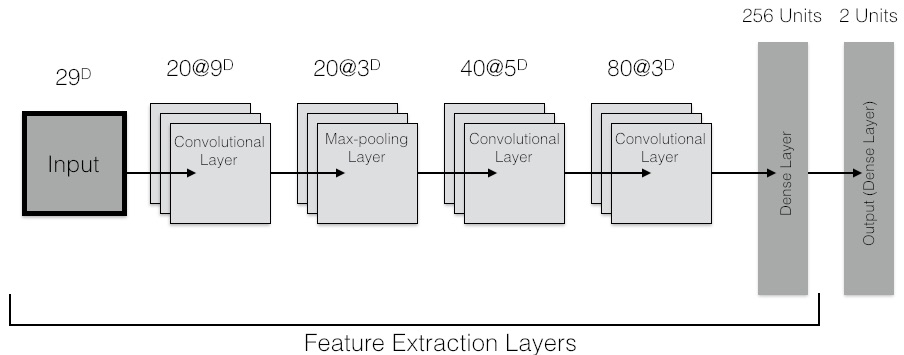
\includegraphics[width=1\textwidth]{architecture.jpg}
\caption[An overview of the CNN architecture used in experiments presented in this report]{Diagram showing an overview of the basic network architecture used in all experiments. In some cases more than one feature extraction layer will be used, with an additional concatenation layer between the dense layer and output. D denotes the dimensionality of the input and the filters, which are used in both 2 and 3 dimensions. The numbers above the hidden layers indicate the number of feature maps generated and the size of the filter. For example 20@$9D$ indicates there are 20 feature maps, sharing $9^D$ weights}
\label{fig:Network}
\end{figure}
 
The profile of the network resembles that of Prasoon et al. exactly, with one max-pooling layer following the first convolution, followed by two convolutional layers. This is of particular importance to our specific problem which is looking at very thin cartilage structures. By incorporating too many pooling layers when looking at such a small structure, the features may be over-summarised, leading to a loss in signal.  \\
 
Filter sizes are chosen here which decrease in size from $9^{D}$ to $5^{D}$ to $3^{D}$. This is with an aim to capture larger structures in earlier layers, whilst the layers closer to the output with smaller filters aim to capture finer structures. This is in contrast to the implementation seen in the implementation by Prasoon et al. \cite{Prasoon2013DeepNetwork}, which uses a fixed filter size of $5^{2}$ for all layers. For all layers, a ReLu activation function is used. \\

Batchwise training is used to load groups of patches into the network in a randomised order. All sampled patches are split into $N$ mini-batches, and each mini-batch is then used for training, using categorical cross entropy to measure loss. Nesterov accelerated gradient learning algorithm is then used with back-propagation to update the weights of all layers. An L-BFGS optimisation function was used by Prasoon et al., the details of which we will not go into. Each mini-batch size, learning rate and momentum were tuned for each network.\\

As there are numerous differences between this implementation and that of Prasoon et al., this is not an attempt to directly replicate the results seen there, but merely take inspiration from the work.

\section{Input Configurations}
Image segmentation through voxel-wise classification requires the design of input vectors which sufficiently describe the voxel in question. This requires that enough information is captured to enable the best possible separation of classes by the network, whilst having low enough computational demand to operate. Here, the three different input vectors being explored shall be described, and can be seen in figure \ref{fig:Patches}

\begin{figure}[!htbp]
\centering
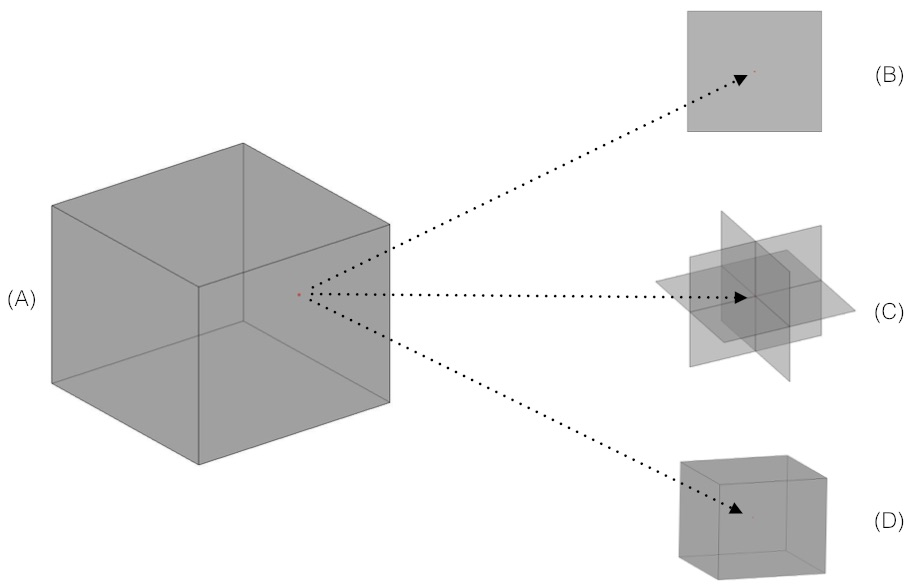
\includegraphics[width =1\textwidth]{patchesA.jpg}
\caption[Illustration of the network inputs extracted from an MRI scan]{Diagram showing overview of the patches used for convolution extracted from an (A) MRI scan in (B) saggital planar, (C) Tri-planar including coronal, saggital and axial planes, and (D) Full 3D, all centred around the voxel to be classified.}
\label{fig:Patches}
\end{figure}

\subsection{2D Planar Approach}
The first convolutional network uses a single 2-dimensional patch centred around the voxel to be classified. Using the saggital slices of the image, 29x29 square patches are extracted using NumPy, and fed into the network architecture which is outlined in Figure \ref{fig:Network}.\\

Although there is little spatial information provided here in a single plane, due to the small amount information provided, there are fewer parameters to optimise, meaning fewer degrees of freedom. This should allow faster computational speed. For training this network, a learning rate of $1.0*e\textsuperscript{-6}$ was used, a momentum of 0.9, and batch size of 250 patches.

\subsection{Tri-Planar Approach}
The second approach is an adapted structure to that of Prasoon et al., with many of the differences being outlined in Section 4.3. In order to provide some extra spatial information, coronal and axial 2D planes are extracted as well as the saggital plane. This can be seen in Figure \ref{fig:Patches}C. 2D convolutions are then carried out on each patch. \\

Each patch is fed into its own network, resembling the "Feature Extraction Layers" in Figure\ref{fig:Network}. Following the dense layer in each of the networks, a concatenation layer then combines all weights together, before classifying the voxel using a softmax in the output layer. This approach aims to reduce the computational complexity of a full three-dimensional patch, whilst still capturing information in all three planes. For training this network, a learning rate of $1.0*e\textsuperscript{-5}$ was used, a momentum of 0.8, and batch size of 250 patches. 




\subsection{Three Dimensional Approach}
The final approach being explored uses full three dimensional patches and convolutions. This approach is slightly more intuitive given the 3D nature of MRI scans. These patches will also contain much more locally spatial information about the voxel being classified. This does however come at the cost of having many more parameters to be optimised. This may need a longer training time to achieve the optimal parameters, however the number of epochs will be fixed for all experiments, to keep some continuity, although 'wall-clock' time will most likely be longer. For training this network, a learning rate of $1.0*e\textsuperscript{-6}$ was used, a momentum of 0.9, and batch size of 250 patches.


\section{Post-Processing}
One post processing step will be taken in an attempt to improve the accuracy of the classifier. The medial tibal cartilage is a solid structure, comprised of one piece of soft tissue \cite{Majumdar2010AdvancesOsteoarthritis}. With this is mind, the aim will be for the classifier to segment one structure for each class being identified. In order to correct for any classification errors, a Matlab \cite{MATLAB:2010} implementation of the largest connected component algorithm will be used to identify the largest structure in the segmented image, and discard the rest. In the case of $n$ structures are being segmented, $n$ largest connected components will be kept. This assumes a certain level of accuracy from the classifier to ensure there are not larger connected components present. 

\section{Evaluation Strategy}
In order to evaluate the performance of each of the networks, Dice-Sørensen Coefficient (DSC) \cite{Zou2004StatisticalIndex.}, Equation \ref{eq=DSC} will be used. This can be seen as the spatial volume overlap of two data sets, and is used widely across image segmentation problems. DSC is given by \\

\begin{equation}
DSC = \frac{2TP}{2TP + FP + FN}
\label{eq=DSC}  \enspace,
\end{equation}\\
where TP (true positive) is the number of correctly identified foreground voxels, FP (false positive) the number of background voxels incorrectly identified as foreground, and FN (false negative) the number of foreground voxels incorrectly identified as background voxels.\\

Sensitivity and specificity will also be measured in the segmentations before post processing is applied. \\


\begin{equation}
Sensitivity =  \frac{ TP }{ TP + FN} 
\label{eq=sens}
\end{equation}
 
\begin{equation}
Specificity  =  \frac{ TP}{ TP + FP} 
\label{eq=spec}
\end{equation}
\\

For a number of subjects, two scans were available, taken one week apart from each other. In order to be able to detect progression of OA in a knee, difference in cartilage volume should be measured accurately after a prolonged period of time such as 1 year. By measuring the volume cartilage from knee scans taken just 1 week apart, a small difference in volume indicates the robustness of a segmentation algorithm. This can be measured by root mean squared coefficient of variation CV(RMSD), expressing the precision. This can be seen in Equations \ref{RMSD} and \ref{RMSD CV}

\begin{equation}
RMSD = \sqrt{\frac{\sum \left ( x_{i} - \hat{x}_{i}  \right )^{2}}{N}}\enspace,
\label{RMSD}
\end{equation}

\begin{equation}
Precision \enspace (CV(RMSD)) = \frac{RMSD}{\bar{x}}\enspace,
\label{RMSD CV}
\end{equation}

where $x_{i}$ is the original volume measurement, $\hat{x}_{i}$ is the re-scan volume measurement, and $\bar{x}$ is the mean of all original volume measurements.\\


All of these measures have also been reported in publications of state-of-the-art methodologies which will allow direct comparison of results. A Student's T-Test will be used to measure if there is a significant difference in DSC scores between the three network architectures and State-of-the-Art methods using the same dataset.

\clearpage

\chapter{Experimentation and Results}
\section{CCBR Data}
Using scans provided by the Centre for Clinical and Basic Research (CCBR) in Ballerup, Denmark, different architectures were evaluated and compared. This was the same dataset used by Prasoon et al. \cite{Prasoon2013DeepNetwork} and Dam et al. \cite{Dam2015} in their segmentation work.

\subsection{Experimental Set Up}
For this study, 140 MR images were used of left and right knees which had been graded by severity of OA by a radiologist. The population was of age 56 \(\pm\) 16, with a body mass index (BMI) of 26\(\pm\) 4 kg/m\textsuperscript{2}, and 47\% were female. Scans were obtained using an Esaote 0.18T C-span scanner. which yielded Turbo 3D T1 sequences. The resolution of the images obtained was 0.7 x 0.7 mm\textsuperscript{2}, with a distance within the range of 0.7 - 0.94 mm between slices. An example of one slice of a scan can be seen in Figure \ref{compare}(g). \\ 

The images were split into 25 training scans, with five kept aside for validation. The remaining 110 scans were kept for evaluation of each network's performance. The division of these test and training scans is the same as the one used by Dam et al. in \cite{Dam2015}.\\

Using the 25 training images and 5 validation images, parameters such as learning rate, momentum and batch size  were tuned and selected for each network configuration. Graphs of both training and validation loss were plotted to observe possible instances of over-fitting. These graphs can be seen in \ref{fig:loss}.\\


\begin{figure}[!ht]
\centering
\begin{tabular}{c}
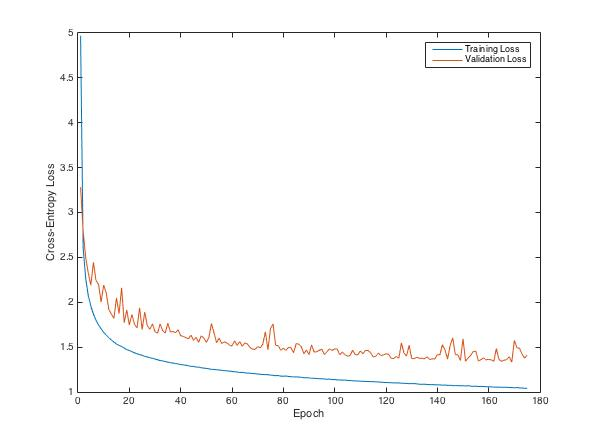
\includegraphics[height = 65mm]{plan_loss.jpg}\\
(a) Planar \\
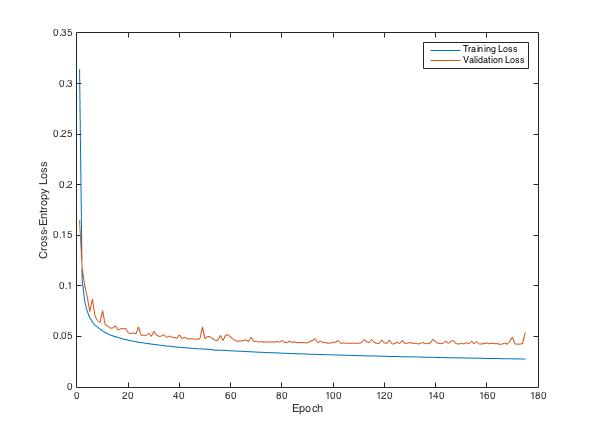
\includegraphics[height = 65mm]{Tri_loss.jpg}\\
 (b) Tri-Planar \\
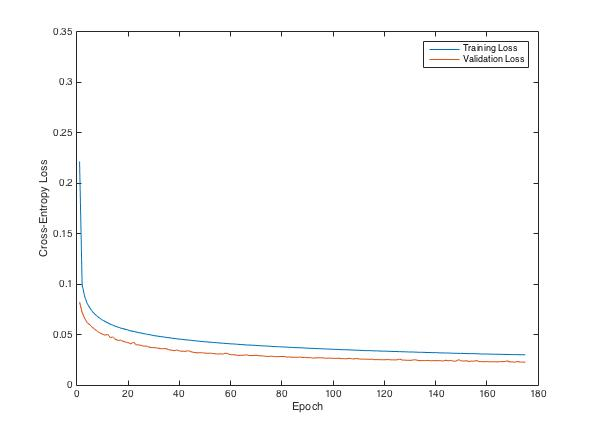
\includegraphics[height = 65mm]{three-loss.jpg} \\
 (c) 3D \\

\end{tabular}
\caption[Graphs of cross-entropy loss for training and validation of CNNs using CCBR data]{Graphs showing the training (blue) and validation (orange) loss for (a) Planar (b) Tri-Planar and (c) 3D network architectures over the complete training period, 175 epochs.}
\label{fig:loss}
\end{figure}


It must be noted that for planar and tri-planar networks, the validation loss stayed slightly above the training loss, which is to be expected. The 3D network however shows the validation loss constantly below the training loss.

\subsection{Results}
\subsubsection{Segmentation Accuracy}
The results of the segmentation of the medial tibial cartilage for the 110 test images can be seen in Table \ref{table:Dice}. It is possible to see that before post-processing the 3D architecture performs significantly better than both planar and tri-planar with a DSC of 0.5653 $\pm$ 0.06367 (P-Value of \textless 0.0001 for both). The tri-planar network performs significantly better than planar and 3D networks post processing with a mean LCC DSC of 0.8707 $\pm$ 0.0474 (P-Values \textless 0.0001 and 0.0013 respectively).\\ 

The distribution of the Dice-Sørensen scores for each network before and after post-processing can  be seen in the box plots in Figure \ref{table:boxy}. It is clear there are extreme outliers for both planar and 3D networks following post processing with DSC scores of 0.\\

The training scans were also segmented and scored in the same way in order to identify any overfitting to the training data. The mean DSC scores for this can also be seen in Table \ref{table:Dice}. \\

An example of a segmentation after CNN and post processing can be seen in Figure \ref{compare}. The scan shown had the median LCC-DSC for the tri-planar network. This figure clearly illustrates the difference in DSC between the three network architectures. \\

\begin{figure}[!h]
\begin{adjustwidth}{-1.5cm}{}
\begin{subfigure}{0.6\textwidth}
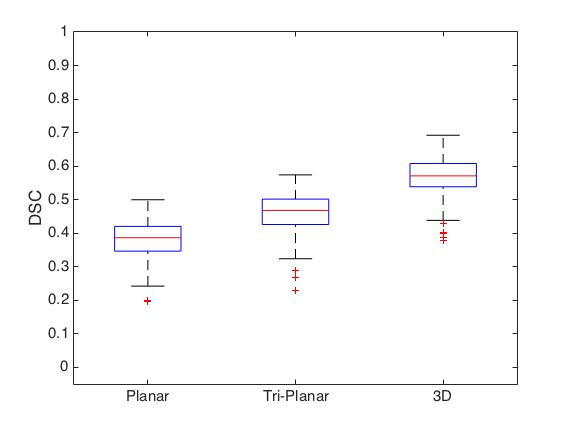
\includegraphics[width=1.1\linewidth, height=7cm]{boxcnn.jpg} 
\caption{CNN}
\label{fig:CNND}
\end{subfigure}
\begin{subfigure}{0.6\textwidth}
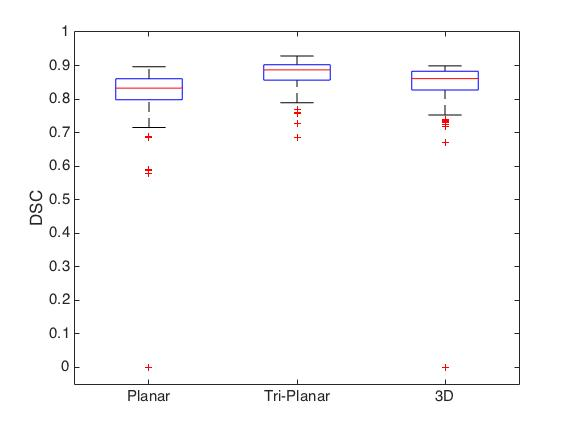
\includegraphics[width=1.1\linewidth, height=7cm]{boxlcc.jpg}
\caption{CNN-LCC}
\label{fig:LCCD}
\end{subfigure}
 \end{adjustwidth}
\caption[Boxplots showing the distribution of DSC scores for each CNN architecture]{Boxplots showing the distribution of DSC scores (a) following CNN classification and (b) after LCC post processing for planar, tri-planar and 3D configurations.}
\label{table:boxy}
\end{figure}

\begin{landscape}
\begin{center}

\begin{table}
\centering
	\vspace{4cm}
   \caption[Results of MRI segmentation for all network architectures used]{Mean DSC, sensitivity and specificity scores for the segmentation of the medial tibial compartment of knee MRI scans using, tri-planar and planar network configurations, as well as DSC after using Largest Connected Component post processing. }
\begin{tabular}{|c|c|c|c|c|c|c|}

\hline

           & Mean DSC            & Median DSC & Mean Spec           & Mean Sens           & Mean LCC-DSC        & Median LCC-DSC \\ \hline
Planar     & 0.3779 $\pm$  0.0589 & 0.3864     & 0.9966 $\pm$ 0.0005 & 0.7598 $\pm$ 0.0699 & 0.8037 $\pm$ 0.1253 & 0.8326         \\ \hline
Planar Training & 0.3965 $\pm$ 0.0517	& 0.3916  &	 0.9965 $\pm$ 0.0005	& 0.7874 $\pm$ 0.0700 &	0.8460 $\pm$ 0.0476 	  &	             0.8520		 	  \\ \hline
Tri-Planar & 0.4596 $\pm$ 0.0656 & 0.4680     & 0.9972 $\pm$ 0.0004 & \textbf{0.8534 $\pm$ 0.0583} & \textbf{0.8707 $\pm$ 0.0474} & \textbf{0.8872}         \\ \hline
Tri-Planar Training & 0.4859 $\pm$ 0.0505	& 0.4745  &	 0.9972 $\pm$ 0.0003	& 0.8917 $\pm$ 0.0431 &	0.9063 $\pm$ 0.0287 	  &	             0.9136		 	  \\ \hline


3D         & \textbf{0.5653 $\pm$ 0.0637} & \textbf{0.5707}     & \textbf{0.9984 $\pm$ 0.0003} & 0.8053 $\pm$ 0.0722 & 0.8378 $\pm$ 0.0946 & 0.8609         \\ \hline
3D Training &	 0.5959	$\pm$ 0.0510	&	 0.5945		&			  0.9984$\pm$ 0.0003	&		 0.8458	$\pm$0.0595		&				0.8807 $\pm$ 0.0405
		&	 0.8919
			\\ \hline

\end{tabular}

\label{table:Dice}

\end{table}
\end{center}
\end{landscape}


\begin{figure}
\centering
\begin{tabular}{cc}
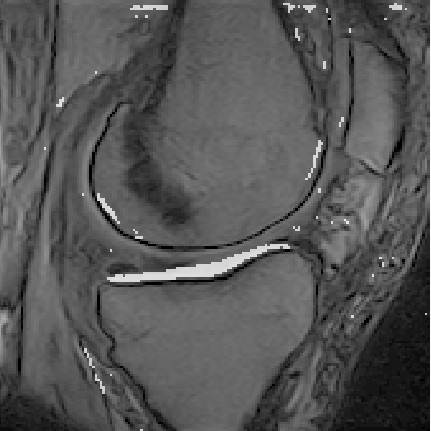
\includegraphics[width = 3.75cm]{planpre.jpeg} & 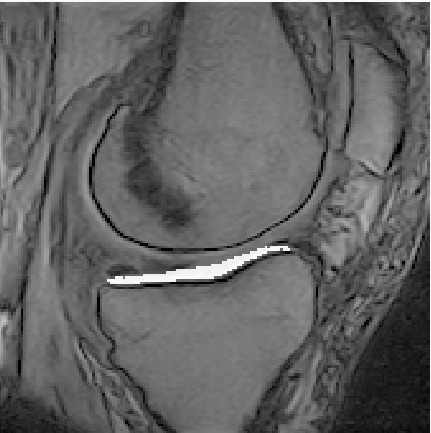
\includegraphics[width = 3.75cm]{planpost.jpeg}\\
(a) Planar Segmentation & (b) Planar Post LCC \\
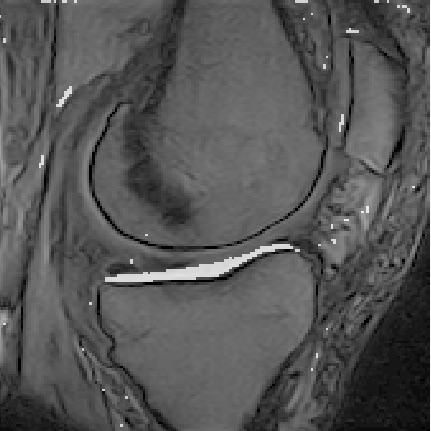
\includegraphics[width = 3.75cm]{tripre.jpeg} & 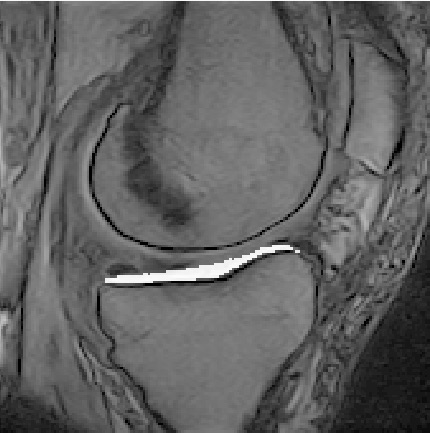
\includegraphics[width = 3.75cm]{tripost.jpeg}\\
(c) Tri-Planar Segmentation & (d) Tri-Planar Post LCC \\
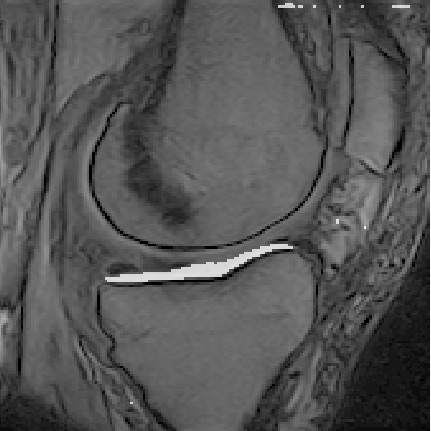
\includegraphics[width = 3.75cm]{3dpre.jpeg} & 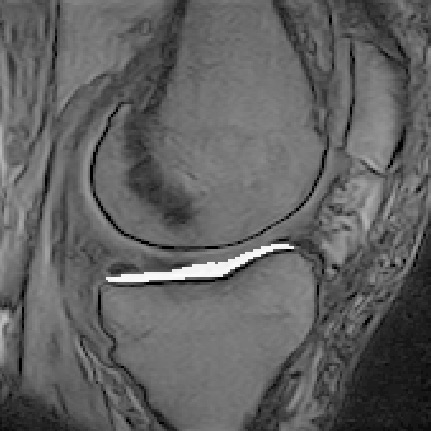
\includegraphics[width = 3.75cm]{3dpost.jpeg}\\
(e) 3D Segmentation & (f) 3D Post LCC \\


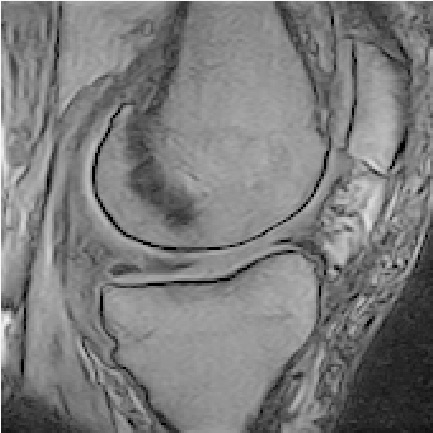
\includegraphics[width = 3.75cm]{natural.jpg} & 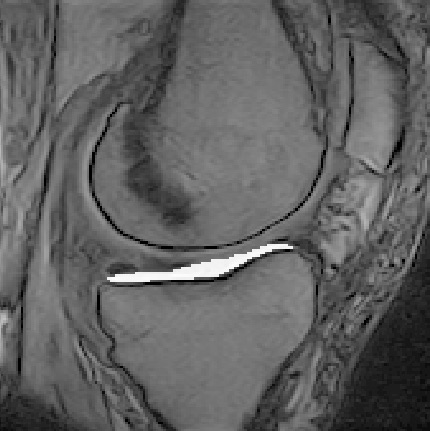
\includegraphics[width = 3.75cm]{labal.jpeg}\\
(g) Original Scan &(h) Manual Segmentation Mask\\
\end{tabular}
\caption[Example of an image before and after segmentation and post-processing]{Images of a saggital slice of a knee MRI with segmentations superimposed on top. These are shown both before and after LCC post processing. The reference mask and original scan have been included for comparison. }
\label{compare}
\end{figure}

\clearpage
\subsubsection{Error Evaluation}
Graphs were plotted to identify the segmentation accuracy of individual images with each network, which can be seen in Figure \ref{lines}.

\begin{figure} [!h]
\centering
\label{subfig:a}
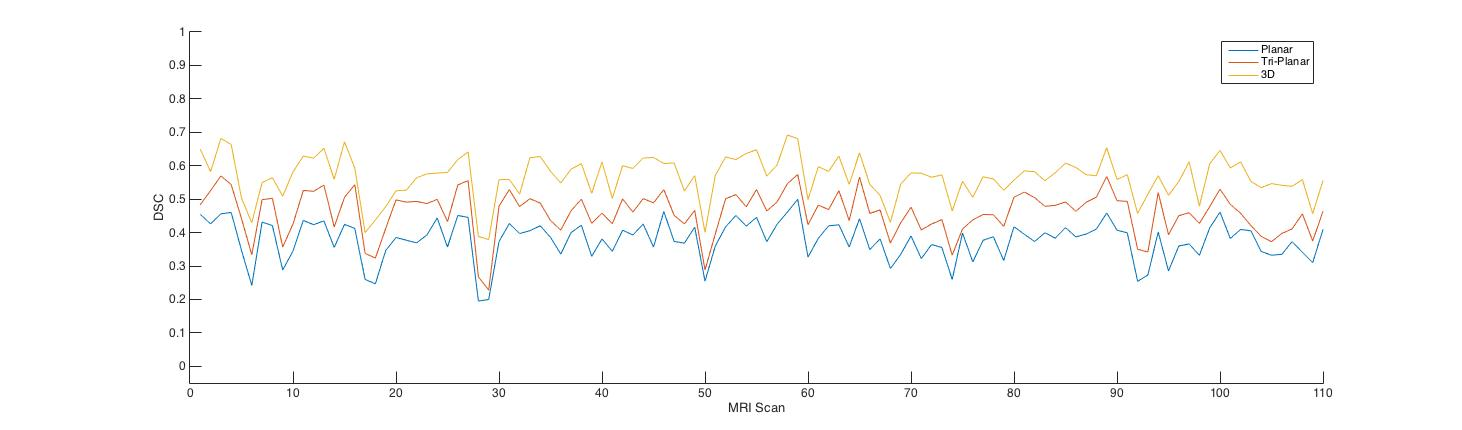
\includegraphics[trim={5cm 0 4cm 0},clip,width=1\textwidth]{Dice_chart.jpg}\\ (a) CNN

\label{subfig:b} 
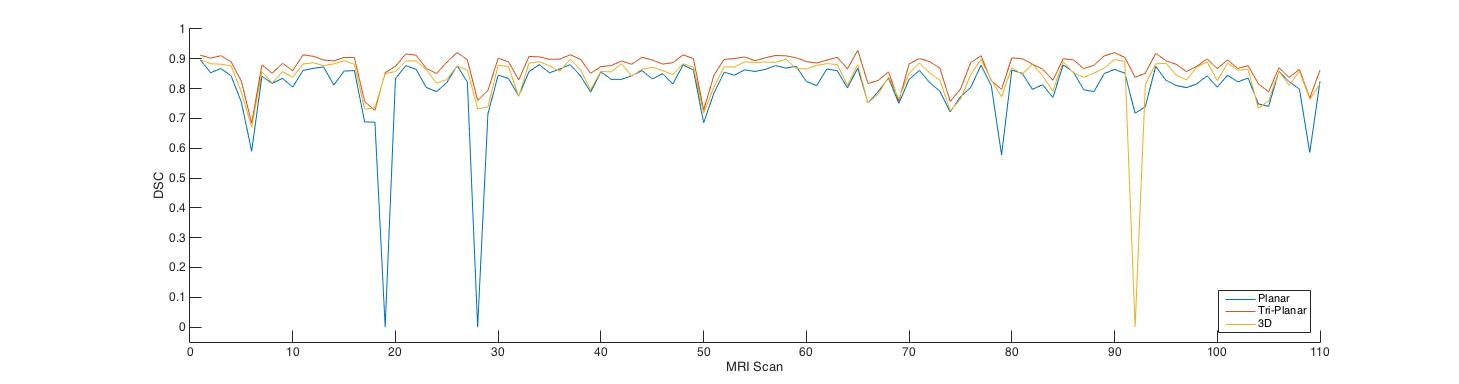
\includegraphics[trim={5cm 0 0 0},clip,width=1.1\textwidth]{LCC_chart.jpg} (b) LCC CNN
\caption[DSC scores shown for each individual MRI scan after CNN segmentation and LCC CNN segmentation]{DSC Score for each MRI scan shown (a) after CNN segmentation and (b) after LCC post processing.}
\label{lines} 

\end{figure}

There appears to be a correlation between a certain image having a low DSC score with all three tests. To investigate a possible cause of this, the mean DSC was calculated for healthy knees and diseased knees using the Kellgren-Lawrence grade provided. A Wilcoxon Rank Sum test was then used to highlight the significance between the two groups for each network. \\

Two of the worst cases of segmentation can be seen in Figure \ref{plane-bad} and \ref{3d-bad}. It is clear from both visualisations that the medial tibial cartilage has been segmented somewhat successfully, however in post processing, these compartments have been lost resulting in a DSC score of 0. These are both extreme cases and not representative of the rest of the segmentation. 


\begin{table}[!h]

\centering
\caption[DSC scores for healthy knees compared to diseased knees]{Mean DSC scores for planar, tri-planar and 3D architectures split into two groups - Healthy Knees, those with a Kellgren-Lawrence(KL) score of 0, and diseased knees, those with a KL score of 1 or greater. P-Values calculated using Wilcoxon Rank Sum test, show statistical significance of difference between the two means. }
\begin{tabular}{|l|l|l|l|}
\hline
 & Healthy Knee DSC      & Knee with OA & P-Value         \\ 
 & (KL = 0, 50 patients) & (KL \textgreater 0, 60 patients) & \\ \hline
Planar                   & 0.8429 $\pm$ 0.0371                  & 0.7710 $\pm$ 0.1596                             & $6.26e^{-06}$         \\ \hline
tri-planar                & 0.8945 $\pm$ 0.0212                  & 0.8509 $\pm$ 0.0539                             & $2.25e^{-07}$ \\ \hline
3D                       & 0.8526 $\pm$ 0.1253                  & 0.8254 $\pm$ 0.0563                             & 0.0039         \\ \hline
\end{tabular}

\label{table:KL}
\end{table}




\begin{figure}[!h]
\centering
 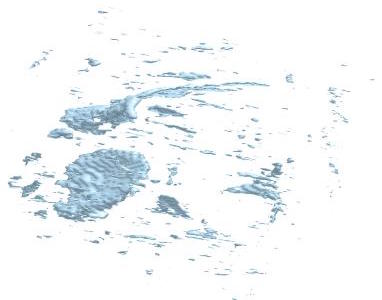
\includegraphics[width=120mm]{plan-seg.jpg}\\
 \centering
 (a) Tibial Cartilage Segmentation with 2D Planar CNN\\
 \begin{adjustwidth}{-1.5cm}{}
\begin{tabular}{cc}
  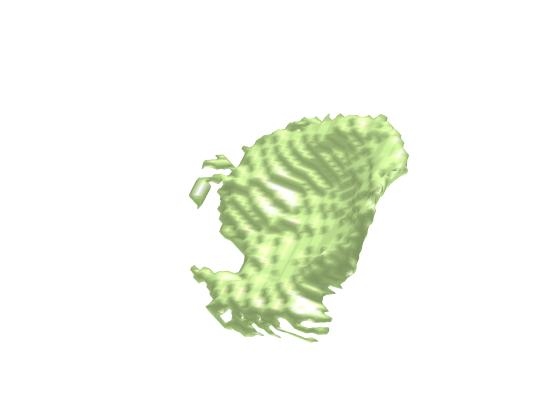
\includegraphics[width=80mm]{lab1.jpg} &   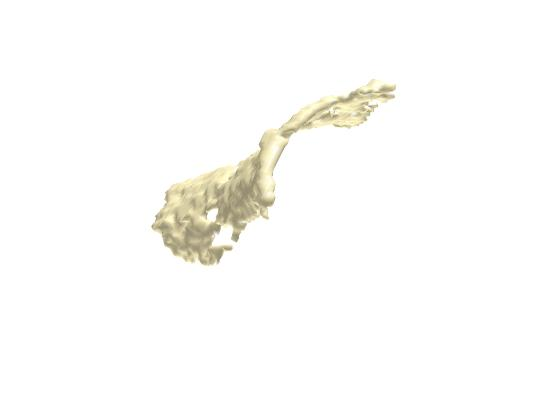
\includegraphics[width=80mm]{planlcc.jpg} \\
(b) Medial Tibial Manual Segmentation & (c) Post Processing with LCC\\

\end{tabular}
\end{adjustwidth}
\caption[Visualisation of medial tibial cartilage segmentation error Using a 2D planar CNN architecture]{Visualisation of an outlier of medial tibial cartilage segmentation using a 2D planar CNN. (a) shows the full image following CNN segmentation, with a structure representative of the (b) manual segmentation in the bottom left hand corner. (c) shows the post processed image after processing with largest connected component removed the medial tibial structure. }
\label{plane-bad}
\end{figure}

\begin{figure}[!h]
 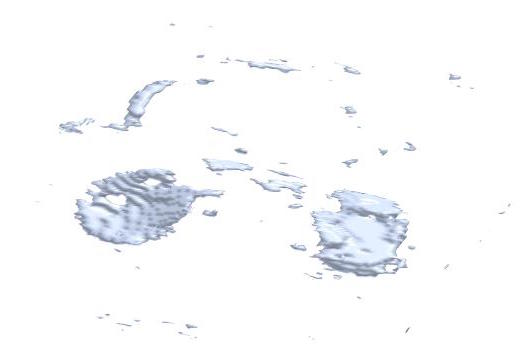
\includegraphics[width=130mm]{3d_seg_worst.jpg}\\
 \centering
  (a) Tibial Cartilage Segmentation with 3D CNN\\
 \begin{tabular}{cc}
  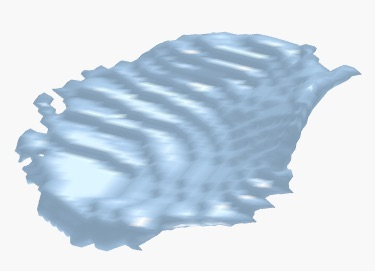
\includegraphics[width=40mm]{3dlab.jpeg} &   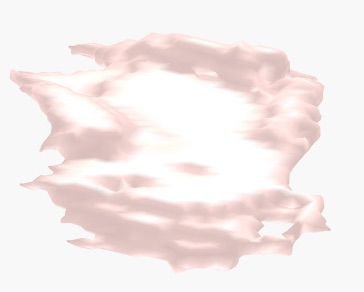
\includegraphics[width=40mm]{3derror.jpeg} \\
(b) Medial Tibial Manual Segmentation & (c) Post Processing with LCC\\

\end{tabular}

\caption[Visualisation of medial tibial cartilage segmentation error using a 3D CNN architecture]{Visualisation of a segmentation error with a 3D CNN network. Here the lateral tibial cartilage has been segmented as well as the medial tibial cartilage. Due to the larger size of the lateral segment, the medial tibial cartilage was completely removed in post processing resulting in a DSC of 0.}
\label{3d-bad}
\end{figure}

\clearpage

\subsubsection{Computational Cost}
As well as segmentation accuracy, in order to consider computational expenditure the time taken to run each network for 175 epochs (the complete train time) with all 30 training images was measured.

\begin{table}[!ht]
\centering
\caption[Time taken to train each network architecture using CCBR data]{Run times for the training of different network architectures with 110 training scans over 175 training epochs}
\begin{tabular}{|c|c|c|c|}
\hline
 & Real Time   & User Time   & System Time \\ \hline
Planar                   & 188m 37.9s  & 166m 36.2s  & 22m 15.5s   \\ \hline
tri-planar                & 303m 17.3s  & 250m 49.0s  & 52m 44.8s   \\ \hline
3D                       & 2085m 15.9s & 1750m 10.3s & 337m 6.6s   \\ \hline
\end{tabular}
\label{time}
\end{table}

The time taken to segment an individual scan was also measured for each network, with time being averaged over all 110 training scans. These times can be seen in Table \ref{seg_time}.

\begin{table}[!ht]
\centering
\caption[Average time taken to segment an image using each network architecture using CCBR data]{The average time taken to segment a full MRI scan using each of the architectures is shown here. The average was made over the same 110 test scans in each case.}
\begin{tabular}{|c|c|c|c|}
\hline
 & Real Time   & User Time   & System Time \\ \hline
Planar                   & 2m 8.5s & 1m 57s    &  1.17s    \\ \hline
tri-planar                & 2m 37.8s  & 2m 23s  & 14.23s   \\ \hline
3D                       &  27m 7s& 22m 9s & 4m 72s\\ \hline
\end{tabular}


\label{seg_time}

\end{table}

\subsubsection{Multi-Compartment Segmentation}
The manual segmentations provided with each scan included medial femoral cartilage and tibia as well as the medial tibial cartilage. The tri-planar network was adapted to a multi-class classifier used to segment the medial femoral cartilage as well as tibial cartilage. Only the tri-planar network was tested based on performances of previous experiments. The results can be seen in Table \ref{compz}. The same images were used here to train and evaluate the network as in previous experiments. Although the Mean LCC-DSC of the medial tibial cartilage is lower here than in the binary network, it is not significantly so (P-Value, 0.1332).\\

\begin{landscape}

\begin{table}[!ht]
\vspace{4cm}
\centering\caption[Segmentation accuracy for a multi-class convolutional neural network]{Mean DSC, Sensitivity, Specificity and LCC DSC scores for medial tibial and medial femoral cartilage compartments using a multi-class tri-planar convolutional neural network. }
\begin{tabular}{|c|c|c|c|c|c|c|}
           \hline     & Mean DSC & Median DSC & Mean Spec & Mean Sens & Mean LCC DSC & Median LCC DSC \\  \hline
Medial Tibial  & 0.5989 $\pm$ 0.0636 & 0.6096 & 0.9986  $\pm$ 0.0002   &   0.8216  $\pm$ 0.0636 & 0.8593  $\pm$ 0.0478     & 0.8751         \\  \hline
Medial Femoral & 0.326 $\pm$ 0.051  & 0.3286  &   0.9862  $\pm$  0.0020  &    0.0117  $\pm$ 0.0157  & 0.4490  $\pm$ 0.0615     & 0.4477       \\ \hline
\end{tabular}

\label{compz}
\end{table}
\end{landscape}


\begin{figure}[!h]
 \centering
 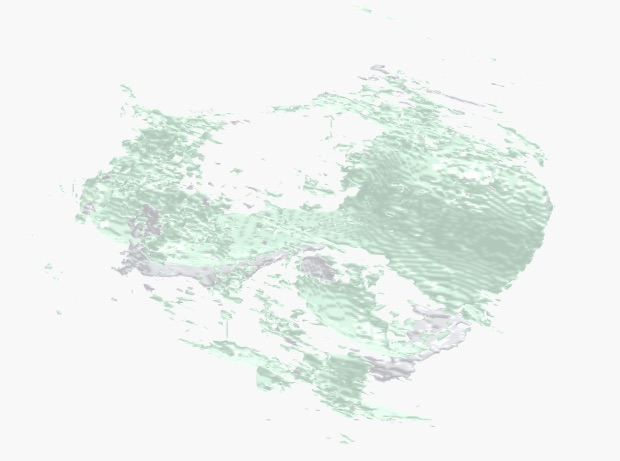
\includegraphics[width=110mm]{comppre.jpeg}\\

  (a) Tibial and Femoral Cartilage Segmentation with a tri-planar CNN\\
   \vspace{1cm}
 \begin{tabular}{cc}

  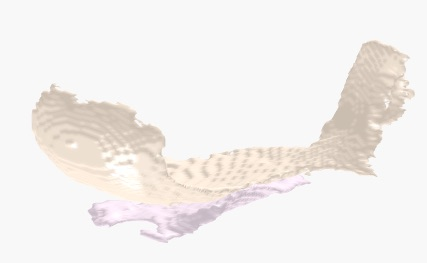
\includegraphics[height=30mm]{label.jpeg} &   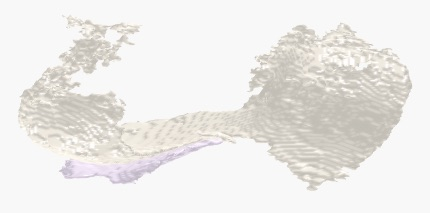
\includegraphics[height=30mm]{compz2.jpeg} \\
(b) Manual Segmentation & (c) Post Processing with LCC\\

\end{tabular}

\caption[Visualisation of tibial and femoral cartilage segmentation using a multi-class CNN]{Visualisation of the median scoring segmentation using a tri-planar multi-class classifier before and after post processing, as well as the manual segmentation used as a reference mask. }
\label{compim}
\end{figure}
\clearpage
\subsubsection{Segmentation Precision}
 
Extra scans were provided for certain patients, which had been acquired one week following the initial scan. Using these scans the precision of each of the classification methodologies could be calculated, identifying percentage change in cartilage volume between the two scans. As no volume decrease should be expected over one week, the objective is to have a zero percent change in cartilage volume between the two scans. The results of these calculations can be seen in Table \ref{RMSDCV}

\begin{table}[!h]
\centering
\caption[Presicion of cartilage segmentation for all CNN architectures]{CV(RMSD) Precision of cartilage volumes for all 38 samples with a rescans, which had been acquired approximately 1 week after the original. }

\label{RMSDCV}
\begin{tabular}{|c|c|}
\hline
                  & CV(RMSD) (\%) \\ \hline
Manual Segmentation & 4.54         \\ \hline
Planar            & 18.26        \\ \hline
Tri-planar        & 5.35         \\ \hline
3D                & 13.51        \\ \hline
Dam et al.        & 4.9          \\ \hline
\end{tabular}
\end{table}

\section{Segmentation Challenge}
This year, the International Workshop on Osteoarthritis Imaging \cite{2016InternationalChallenge} hosted a segmentation challenge, welcoming all fully- and semi-automated segmentation routines to enter and compete against others. Although this took place during an early stage of my thesis, with development not quite complete, an entry was made using the framework running at the time. Five teams in total took part (including this entry), with all other entries adopting a multi-atlas based approach. The set up and results can be seen in the following sections.

\subsection{Experimental Set Up}
After exclusion of two scans with problematic segmentation masks, there were 28 training DESS sequence images, acquired at 3T, which were 0.6mm in isotropic resolution and contained 160 slices over the entire knee. The scans were in DICOM format  along with reference masks with manual segmentations of both femoral and tibial cartilage. There were also 14 images provided without reference masks for evaluation. \\

The standard pre-processing methodology was used for patch generation in preparation for training as outlined in section 4.1. Five images were kept aside for validation of the network and to enable robust parameter selection. Here, rather than 1 compartment being segmented, there were three. The labels were split into femoral cartilage and tibial cartilage, with the latter being made up of two separate structures with the same label.

\subsection{Architecture}
A slightly different architecture was employed here, with multiple full 3D patches used, with an additional spatial prior included. This can be seen in Figure \ref{challenge arch}. Two 3D patches of size $5^3$ and $9^3$ were fed into the two separate networks for convolution. Due to the small size of the patches being used, no pooling layers were used at all. An extra feed forward network was added which took an input of the $x$, $y$, $z$ coordinates of the voxel being classified. This was an attempt to add some spatial information into the network. \\


\begin{figure}[!h]
\centering
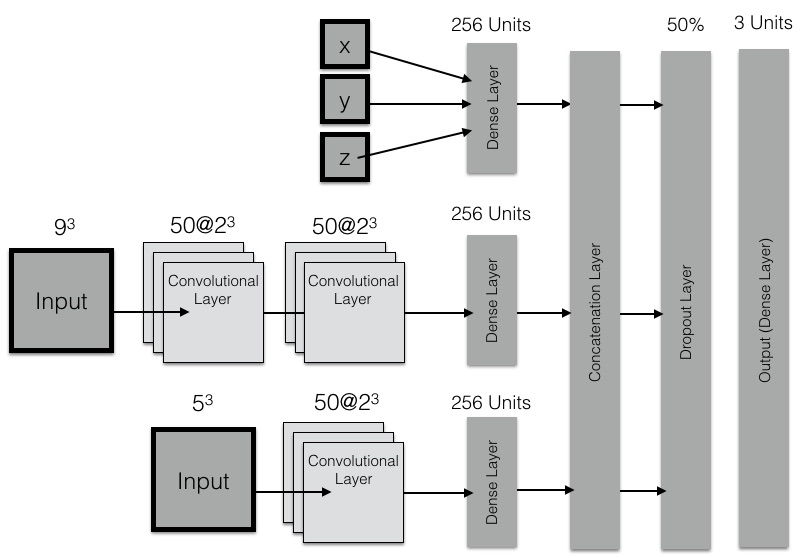
\includegraphics[height = 6.5cm]{arch2.jpg}
\caption[An overview of the architecture used in the IWOAI Segmentation Challenge]{Depiction of the architecture used in the IWOAI 2016 Segmentation Challenge. This consisted of 3 separate networks; a Feed Forward neural network with inputs being defined by the $x$, $y$, $z$ coordinates of the voxel being classified, a CNN with $9^3$ patch input, and a CNN with $5^3$ patch input. These are all concatenated before being fed into a drop-out layer before finally the output layer.}
\label{challenge arch}
\end{figure}

For both of these networks, 20 feature maps were generated at each convolutional layer, with a filter size of 2x2x2. In this set up, only 50 training epoch were used, however a larger batch size of 500 was used, and a learning rate and momentum of 0.001 and 0.8 respectively. The cross-entropy loss over all 50 training epochs can be seen in Figure \ref{challtrain}.\\

Post processing was slightly different for the challenge data. This began with rigid registration, where each training scan was registered onto the evaluation scan which was provided by Erik Dam. Using a multi-atlas created from the registered mask, voxels with no cartilage overlap from any training scan were classified as being background and the output from the neural network was discarded.\\

Using the already "cleaned" segmented images, largest connected component algorithm was used to select three largest connected segments, one was selected for the femoral cartilage, and two for the tibial cartilage. 

\begin{figure}
\centering
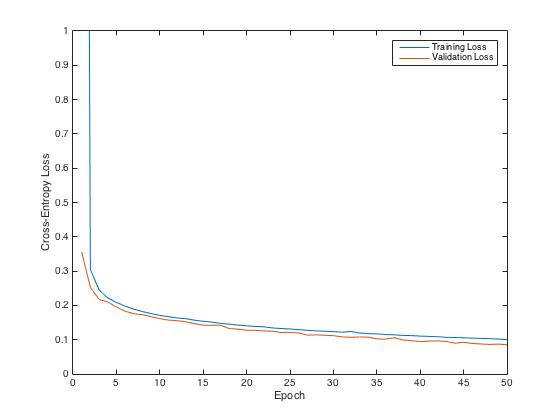
\includegraphics[width=10cm]{challloss.jpg}
\caption[Graph of cross-entropy loss for training and validation datasets for the IWOAI Segmentation Challenge]{Figure showing training and validation cross entropy loss for a CNN architecture used for segmentation of tibial and femoral cartilage }
\label{challtrain}
\end{figure}




\subsection{Results}

Unfortunately, no labels were provided for the evaluation scans, meaning that an in depth analysis could not be done. The scores of the full training set can be seen in Table \ref{table:chall}.\\

\begin{table}[!h]
\centering
\caption[DSC Scores for the training data provided for the IWOAI Segmentation Challenge]{Table of mean Dice scores and standard deviations at different stages of segmentation. These scores are the average over all training images segmented, after training with the same set of images.}
\begin{tabular}{|c|c|c|c|}
\hline
                          & Femoral Mean DSC  & Tibial Mean DSC \\ \hline
CNN                       & 0.5424  $\pm$     0.0821     & 0.7060  $\pm$   0.0750   \\\hline
CNN + registration         & 0.7850 $\pm$    0.0778     & 0.7660   $\pm$    0.0685   \\ \hline
CNN + registration + LCC   & 0.7914 $\pm$    0.0787     & 0.7719   $\pm$    0.0704   \\ \hline


\end{tabular}

\label{table:chall}
\end{table}

The DSC of the evaluation scans were calculated in separate regions of the image, as well as for each complete section. Table \ref{results} shows the DSC score for the whole femoral cartilage and tibial cartilage regions for each team. \\

\begin{table}[!h]
\centering
\caption[DSC scores for each team entered into the IWOAI Segmentation Challenge]{Segmentation challenge results showing the mean DSC score for femoral and tibial cartilage segmentation. 'Deep In Progress' was the team name of the CNN architecture described here.}

\begin{tabular}{|c|c|c|}
\hline
Team Name                 & Femoral Mean DSC & Tibial Mean DSC  \\ \hline
BIGR                      & 0.74799          & 0.75982          \\ \hline
BioMediq Shape            & 0.85362          & 0.863            \\ \hline
BioMediq Texture          & 0.85467          & 0.86268          \\ \hline
CombiVTT                  & 0.784            & 0.20053          \\ \hline
\textbf{Deep in Progress} & \textbf{0.84416} & \textbf{0.83202} \\ \hline
\end{tabular}

\label{results}
\end{table}

An example of a scan from this dataset before and after segmentation can be seen in Figure \ref{challll}. 

\begin{figure}[!ht]
\centering
\begin{tabular}{cc}

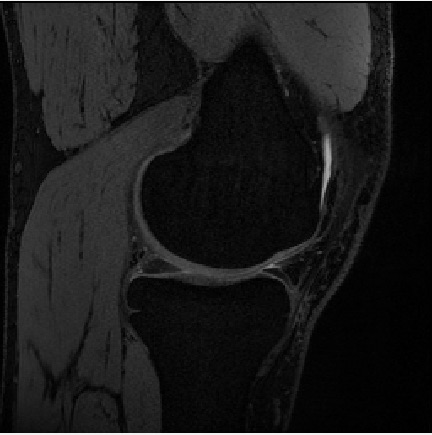
\includegraphics[width=5cm]{rawchal.jpeg} & 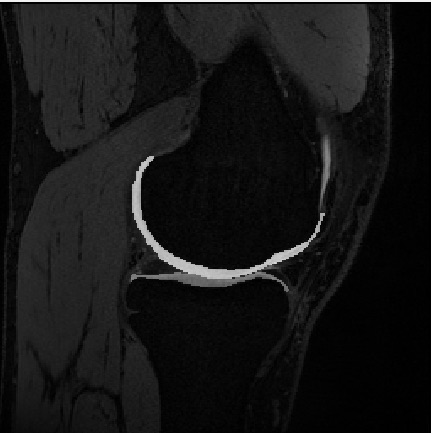
\includegraphics[width=5cm]{challab.jpeg} \\
(a) Raw MRI Scan &  (b) Manual Segmentation\\
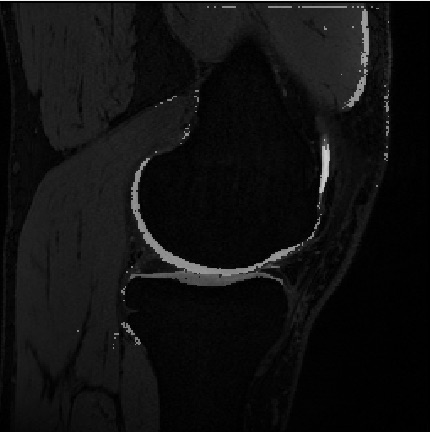
\includegraphics[width=5cm]{segchal.jpeg} & 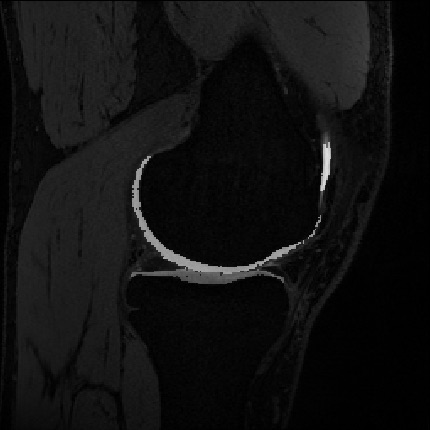
\includegraphics[width=5cm]{segpostchal.jpeg}\\
(c) CNN Segmentation &  (d) Post-processed Segmentation\\

  
\end{tabular}
\caption[An example of an image before and after segmentation and post-processing for the Segmentation Challenge data]{Figure showing a saggital slice of an (a) MRI scan of a knee after (b) Manual Segmentation, (c) CNN Segmentation and (d) after post processing.}
\label{challll}
\end{figure}



\chapter{Discussion}
\section{Network Training}
Before discussing the performance of the network architectures built, it is important to look at the training of all networks to identify possible instances of overfitting. Figure \ref{fig:loss} shows the graphs of cross-entropy loss for the training and validation data sets using planar, tri-planar and 3D architectures. All three graphs show an initial steep decline, during the first 15 epochs, at which point the gradient flattens out, but continues to decrease. There is no point at which the the lines begin to separate, indicating at that no notable overfitting has occurred. The validation curves are also slightly noisier which is to be expected due to the usage of "unseen" data. In accordance to this, planar and tri-planar graphs show that the validation loss is slightly higher then the training loss. This is not however the case for the 3D architecture which shows the training loss to be higher than that of validation.\\ 

A possible explanation for this is the use of mini-batch training, in combination with the large number of parameters needed to be optimised in the 3D network. As the network is trained, the loss for each mini-batch is added to the last, and then averaged over all mini-batches. As the network is training, the parameters will be slightly more optimised than the last meaning the later mini-batches will have a lower loss. The validation set however uses the last set of parameters to calculate the loss, which may result in a slightly lower value, despite the samples having been "unseen". This could be tested and possibly avoided by calculating the validation loss for each mini-batch using the same parameters rather than the final set. Another possible explanation for this disparity could simply be the size of the data sets compared to the number of parameters being optimised in the 3D network, which are much higher than in the 2D networks.   \\

It must be noted that the loss of the planar network, while has a similar loss trajectory as the other two networks, is much higher than the other two networks. The curve for the planar network seems to have a tendency towards one whereas the others tend towards zero. The planar approach utilised the smallest amount data for each voxel being trained - one 2D saggital slice. It may be that this slice was not representative enough of the training voxels to be able to reduce the loss sufficiently, indicating that more information  is needed to sufficiently train the network. \\

\section{Planar, Tri-Planar and 3D Network Evaluation}
Whilst all three networks achieved very respectable DSC scores after post-processing, there were some very clear differences between the performance of each of the networks, with many factors leading to this. As each network was given the same data, the results can be assumed to be indicative of the network itself and not the training data.  \\

The inputs of each network were designed to incorporate varying levels of information, without paying attention to increasing computation time. Here it was important to consider voxels close to that being classified (local), and those further away (global). To some extent, the whole image segmentation score can be seen as a measure of the global spatial preservation, while post processing DSC can be seen as local spatial preservation (classification accuracy of voxels close to the true label).\\

The input of the planar network was the simplest, with only one $29^2$ patch from a saggital slice. This also meant that although the patches in the planar network were of the same dimension as one of the inputs in the tri-planar network, there was no information pertaining to the third dimension. This was somewhat evident from the results seen in Figure 5.3 (a) and Figure 5.5. Whilst it appears that the medial tibial cartilage has been well segmented when compared to the mask, there are a high number of segmentation errors spread across the scan. The sensitivity of this network was also significantly lower at 0.7598 $\pm$ 0.0699 than both tri-planar (0.8534 $\pm$, P-Value \textless 0.0001) and 3D (0.8053 $\pm$ 0.0722, P-Value \textless 0.0001 ) networks which reflects this. This lower number of parameters also meant that there were fewer features which is clear made it hard to successfully classify the voxels. \\ 

By adding two extra planes in both axial and coronal directions to the network, more global spatial context is included, allowing fewer segmentation errors further away from the medial tibial cartilage being segmented. There is also more local information included with this increase in dimensionality. It seemed that this has helped to segment the cartilage segment itself to a higher degree of accuracy. The tri-planar input aimed at including a high level of information, whilst reducing the number of parameters needed to be optimised. This can be expensive, and prone to overfitting. \\

It must also be noted, that due to the arrangement of the tri-planar network, there were many more feature maps generated than in any other architecture tested. Assuming each feature map was learning a different feature, this meant that more features were being learnt and the ability to classify was greater. Despite this, there are still a lot of segmentation errors across the image lowering the DSC.\\

Contrary to this, the 3D architecture had the highest number of parameters to be optimised due to the largest filters being used. The size of the input was also notably larger than the other two networks implemented. This was extremely costly with regards to time taken to train the network, taking more than 10 times longer to train than the planar network, and 14 times longer to segment a single image. This is due to the vast of elements in the patches needed to be generated and convolved. In a clinical setting 27 minutes would be an unacceptable time to have to wait, whilst 3 minutes would be fine. \\ 

From Figure 5.6, it is clear the segmentation by the CNN itself is far better than that of the tri-planar and planar architectures. There are far fewer segmentation errors spread across the image. This resulted in a higher DSC score of 0.5653 $\pm$ 0.0637, significantly higher than that of the planar and tri-planar networks (P-Values both \textless 0.0001).\\

The computational complexity of the 3D network posed a problem in the evaluation of the network given the amount of memory needed. With all three networks, the voxels to be classified had to be split into smaller subsets in order to be able to fit them into the GPU memory. When segmenting the images, the mini-batches had to be more than half the size of that used in planar and 3D networks, creating this time cost. \\

The higher number of parameters also requires a large amount of data to be determined accurately enough. For each network trained, the same number of voxels were sampled and used for training. By increasing the amount of training data used for the 3D network, it is likely the accuracy would also increase. Training with extra data could be problematic with due to the time taken, however as this is a procedure which must only occur once, it is manageable. In order to investigate this, one could investigate the performance of each network trained with a series of different training sizes. For example by increasing and decreasing the number of images used for training, before evaluating each network architecture. This should give an indication of how the performance is dependant on the size of the training data.\\

\section{Post-Processing and Error Correction}

Due to large amounts of segmentation error in all three networks, the Largest Connected Component algorithm was needed to remove unwanted artefacts. As can be seen from the box-plots in Figure \ref{table:boxy}, there is a notable difference between the CNN and post-processed DSC scores. These post-processed DSC scores give a better idea of how accurately the actual medial tibial cartilage segmentation was segmented. \\

Following post-processing, the tri-planar architecture had best performance, with a DSC of 0.8707 $\pm$ 0.0474. This is significantly better than the 3D architecture (DSC 0.08053 $\pm$ 0.0722, P-Value 0.0013) and planar architecture (DSC 0.07598, P-Value \textless 0.0001) It can be seen from Figure 5.4 that its DSC was also consistently highest for almost every image with the exception of some which were surpassed by the 3D architecture. \\

From these charts, each image seems to have a similar DSC score for all three architectures. This indicates that the image itself plays a part in its "ability" to be correctly segmented. This could be due to a number of reasons. As the training set was relatively small, it is possible that the images which score badly are not well represented in the training data. There may also have been a large amount of noise on these images making it difficult to segment them accurately.  \\

Another factor is that diseased knees are more difficult to segment than healthy knees due to pathological changes in the tissue making it more heterogeneous. The DSC scores were split between healthy and diseased for all networks, showing that for planar and tri-planar, the difference between the mean DSC for healthy knees and diseased is certainly significant with a Wilcoxon P-Value of \textless 0.05. This could possibly be corrected by training on many more diseased knees to try and allow for more biological variation. Another way of improving this could perhaps be to increase the number of voxels sampled near the foreground voxels. In the current sampling methodology, all voxels were samples which were adjacent to a labelled voxel. By extending this slightly further, ridge detection may be improved. \\

In order to quantify error more accurately, by mapping the probabilities assigned to each foreground voxel by the classifier, it may be possible to identify if there is a systematic error occurring or perhaps more random segmentation error. It may then be possible to threshold the classifier to exclude voxels that were below a level of certainty.  \\

In three images, post processing a DSC of zero was achieved. In all cases the medial tibial cartilage was identified, however due to the LCC algorithm used this foreground was removed. Figure 5.5 shows one of the cases which occurred using the planar network. There was a large segmentation error in the upper part of the scan which happened to be larger than the cartilage itself. Figure 5.6 shows another case with the 3D architecture. Here the misclassified voxels actually belong to the lateral tibial cartilage compartment which is, on average, larger than the medial component \cite{Teichtahl2012AnthropometryJoint}. These are both examples of how translation invariance has caused segmentation error. \\

Translation invariance is a key principle of convolutional neural networks, due to the sharing of weights and the process of max-pooling. In the case of trying to identify a small cartilage volume located centrally in an image, spatial invariance is not always useful. There is a large amount of spatial information lost during a max-pooling layer when no overlapping windows are used. By incorporating a spatial prior during training, this could potentially be avoided. This was done in the segmentation challenge through he use of $x, y, z$ coordinates. This however does add to the complexity of the network and so may also hinder optimisation of parameters. This was attempted, but due to time constraints was not completed. A simpler approach would be to include more voxels further from the labelled sample.  \\

Using LCC seems to be a good method for correcting segmentation error, however is not very sensitive to identifying the correct segment in the case large errors occur. This could be simply rectified by using a multi-atlas formed from the segmentation masks, and localising the cartilage to this given area as used in the IWOAI Segmentation Challenge.

\section{Multi-class Segmentation}
The same tri-planar architecture used for the medial tibial segmentation was extended to allow for an extra compartment, medial femoral cartilage. This change made the problem slightly more difficult due to the higher number of separation boundaries needed to be constructed \cite{Silla2006Time-SpaceClassification}. This is reflected in the final DSC scores of 0.8593 $\pm$ 0.0478 for medial tibial cartilage and 0.4490 $\pm$ 0.0615 for medial femoral cartilage with post processing. Interestingly however, the DSC from the CNN before post processing is significantly higher for the tibial cartilage (0.5989 $\pm$ 0.0636) than that achieved by the binary classifier (0.4596 $\pm$ 0.0656) with a P-Value of \textless 0.0001. This is possibly due to medial femoral cartilage being larger than the tibial cartilage, and so creating a bias towards voxels being classified into this foreground compartment. This effect can actually be seen in Figure \ref{compim}(a) in which nearly all misclassified voxels belong to the femoral cartilage. As with the tibial cartilage, all femoral cartilage was included in the training data. Due the larger volume of this compartment, there is likely a bias towards this compartment. This could be corrected for by adding a weight to the probabilities obtained by the softmax to adjust for class imbalance.\\

In order to obtain higher dice scores for both compartments, one possible strategy would be to construct a binary classifier for each compartment. This has shown to yield better DSC scores of the tibial cartilage as seen in previous experiments \ref{table:Dice} and likely to have the same effect for the femoral cartilage. It is unlikely however to improve the DSC of the femoral cartilage enough to reach the same level of the tibial compartment classification. \\

The error seen in the segmentation of the femoral cartilage is cartilage belonging to the lateral side of the tissue, which was not labelled. By providing more data samples in this region, it may be possible to correct for this. 


\section{Comparison to State-of-the-Art Methods}
As seen in Section 3.3, many other groups have used various methods to segment tibial cartilage, with three selected results presented in Table \ref{SOA}. Also important to note is that both Dam et al. and Prasoon et al. have used the same CCBR data used in the first experiments in this paper. \\

The first methodology which utilised the same CCBR data set, and so can be used for direct comparison is that of Dam et al. \cite{Dam2015}. Dam reported a mean DSC of 0.846 $\pm$ 0.048, again, significantly lower than that presented here of 0.8707 $\pm$ 0.0474 (P-Value 0.0002). Their methodology used prior knowledge to "hand-craft" features which best distinguish between foreground and background voxels. This is in contrast to the CNN approach which learns the best features possible in order to solve the problem. This may be an explanation for the increase in DSC for tibial segmentation.  \\ 

Precision was also calculated for each of the three network architectures in the same way as in \cite{Dam2015}. The results in  Table \ref{RMSDCV} show that the precision of the tri-planar network, 5.35\%, and thus the robustness of the method, is lower than that of Dam et al. and the manual segmentation.

Prasoon et al. \cite{Prasoon2013DeepNetwork} also used a tri-planar CNN methodology. The results achieved using a tri-planar approach in this report were greater than that achieved by Prasoon et al., of 0.825 $\pm$ 0.043 (P-Value \textless 0.0001). From the documentation published by Prasoon, it appears no post processing steps were used. It is therefore important to identify these differences to potentially further increase the DSC post-processing. There are many differences between the implementation of the two networks, which may have led to this vastly increased CNN segmentation accuracy. What is also interesting, in spite of this, is the fact Prasoon appears to use less than one quarter of the number of training voxels used here, 120,000. \\

The actual architecture of the network is almost identical to the tri-planar network, except for the filter sizes which were slightly altered in this report, and the number of feature maps generated. Prasoon et al. included a slightly higher number of feature maps in the later layers of the network, with 1,792 nodes in the final dense layer. This allows for a larger number of features to be learnt, meaning perhaps more variation can be captured. This may have made a difference to the performance, but it is unlikely to be responsible for the complete increase in DSC. \\

While Prasoon showed that the CNN classification accuracy was significantly higher than all methods shown in this report, the sensitivity reported, 0.819 $\pm$ 0.076, was lower than the 0.8534 $\pm$ 0.0583 achieved using the tri-planar method here. This indicates that the segmentation of the actual cartilage in this report is more accurate, despite many errors across the image which were not reported by Prasoon et al..\\

Zhang et al. \cite{Zhang} actually reported a higher DSC of 0.880 $\pm$ 0.102 for the medial tibial cartilage. This value is the mean over 11 evaluation images. The method used here employed a 2-step SVM-discriminative random field approach, using multi-contrast MR scans. For this method features are specifically designed which incorporate information pertaining to the spatial dependencies of neighbouring voxels. Whilst the DSC score is higher, its difficult to directly compare results due to the vast size difference in data sets, with a data set 10\% of that used here. As a different data set has been used, we not not calculate a P-Value here. \\

\section{Segmentation Challenge}

The architecture for the segmentation challenge was different from the others explored, using two much smaller 3D patches, and a spatial prior. As can be seen from Figure \ref{challll}, there was still a large amount of segmentation error across the image, similar to that seen with the CCBR data, perhaps even to a higher degree. This is unsurprising given the small filter sizes used which do not allow a view of the global spatial environment, and perhaps only give an indication of the local voxels present. There was however the incorporation of a spatial prior in the form of $x$, $y$ and $z$ coordinates of the voxel being classified, although it is not clear how much of an impact this had.\\

The DSC scores achieved of 0.84416 and 0.83202 for the test images were higher than that seen in the multi-class classifier used with larger patches, and was the third highest DSC obtained in the competition. Extra geometric information was included however with the use of a registered multi-atlas to remove unwanted foreground voxels, as well as the LCC algorithm. This step would likely have improved the DSC of both tibial and femoral cartilage in the multi-class classifier. \\

It would be interesting to combine the smaller 3D patches, which are not as costly in terms of time or memory as the big patches, with the tri-planar network configuration. This would combine some level of global information captured by the tri-planar input, as well as the high level of local spatial information provided by the small 3D patches. By registering the images to a reference mask, the impact of a spatial prior be it a coordinate system or something slightly more complex, would likely be more effective. 


\chapter{Conclusion \& Further Work}

This project set out to explore 2D and 3D methodologies for the segmentation of cartilage from MRI scans.  From the results presented, the 2D tri-planar methodology was by far the most successful in its ability to accurately segment tibial medial cartilage with a DSC of 0.8707 $\pm$ 0.0583. It was also a good trade-off between computational cost and performance. Whilst the 3D method was expected outperform the tri-planar approach, the high number of free-parameters present and the amount of training data available was likely the reason this was not the case. \\

The performance of the tri-planar network when compared to existing state-of-the-art methodology had a higher accuracy than those others using the same data set, although precision measurements indicated that this was not quite as robust. This performance was partly due to the geometric transformations using LCC after CNN classification. One conclusion that can be drawn from these experiments is that there seems to be a need for a geometric input or transformation in order to obtain an acceptable performance from the classifier. \\

It is clear that there are many possibilities for further investigation. A more robust data extraction methodology must be used in order to allow for class imbalance and to identify regions of the background which are similar to the foreground. Increasing the depth of the network, number of feature maps and perhaps variations of the input - in essence increasing the complexity of the architecture.\\

There is also likely value in experimenting with different learning algorithms, such as L-BGFS as used by Prasoon et al. \cite{Prasoon2013DeepNetwork}. This algorithm also removes the need for learning rates and momentum to be predetermined, which at times can be difficult to tune. \\

Some experimentation should also be put into modifying the inputs of the networks to incorporate more geometric information. This could done though further experimentation of the coordinate system explored here, or by providing prior probabilities based on a registered multi-atlas. Alternatively, by including input images at different scales, more global information would be included allowing identification of features from further away.
\clearpage

\bibliographystyle{unsrt}
\bibliography{Mendeley.bib}







\end{document}
